\chapter{Nonlinear Analysis Steps}
\label{ch-nonlinear-analysis-steps}





% ******************************************************************
% ******************************************************************
% ******************************************************************
\clearpage
\newpage
\section{Free Field 1D}
\label{free_field_1D}
\paragraph{Elastic Material}
The Real-ESSI input files for elastic example are available 
\href{https://github.com/yuan-energy/Real-ESSI-Short-Course-Examples/tree/master/short-course-examples/nonlinear_analysis_steps/free_field_1D/elastic}{HERE}. 
The compressed package of input files is  
\href{https://github.com/yuan-energy/Real-ESSI-Short-Course-Examples/tree/master/short-course-examples/nonlinear_analysis_steps/free_field_1D/elastic/elastic.tgz?raw=true}{HERE}. 


The Modeling parameters are listed.
\begin{itemize}
  \item Elastic Material Properties 
  \begin{itemize}
    \item Mass Density, $\rho$, \enspace \enspace 2000 $kg/m^3$
    \item Young's modulus, $E$, \enspace \enspace 1.1 GPa
    \item Poisson's ratio, $\nu$, \enspace \enspace 0.1
  \end{itemize}
\end{itemize}





\paragraph{Elastoplastic Material}
The Real-ESSI input files for elastoplastic material example are available 
\href{https://github.com/yuan-energy/Real-ESSI-Short-Course-Examples/tree/master/short-course-examples/nonlinear_analysis_steps/free_field_1D/elastoplastic}{HERE}. 
The compressed package of input files is  
\href{https://github.com/yuan-energy/Real-ESSI-Short-Course-Examples/tree/master/short-course-examples/nonlinear_analysis_steps/free_field_1D/elastoplastic/elastoplastic.tgz?raw=true}{HERE}. 

The Modeling parameters are listed.
\begin{itemize}
  \item von-Mises nonlinear hardening material model 
  \begin{itemize}
    \item Mass density, $\rho$, \enspace \enspace 2000 $kg/m^3$
    \item Young's modulus, $E$, \enspace \enspace 1.1 GPa
    \item Poisson's ratio, $\nu$, \enspace \enspace 0.1
    \item von Mises radius, $k$, \enspace \enspace 60 kPa
    \item nonlinear kinematic hardening rate, $H_a$, \enspace \enspace  30 MPa
    \item nonlinear kinematic hardening rate, $C_r$, \enspace \enspace  25
    \item isotropic hardening rate, $K_{iso}$, \enspace \enspace 0 Pa
  \end{itemize}
\end{itemize}





\begin{figure}[H]
  \centering
  
\includegraphics[width = 0.5cm]{./Figure-files/nonlinear_analysis_steps/free_field_1D/overview.png}
  \caption{Simulation Model}
  \label{fig_decon_1D_motion_1D_model}
\end{figure}

The illustration results of the simulation is shown in Fig.~\ref{fig_decon_1D_motion_1D_model}.
As shown in the results, outside the DRM layer, there is no outgoing waves. 

\begin{figure}[H]
  \centering
  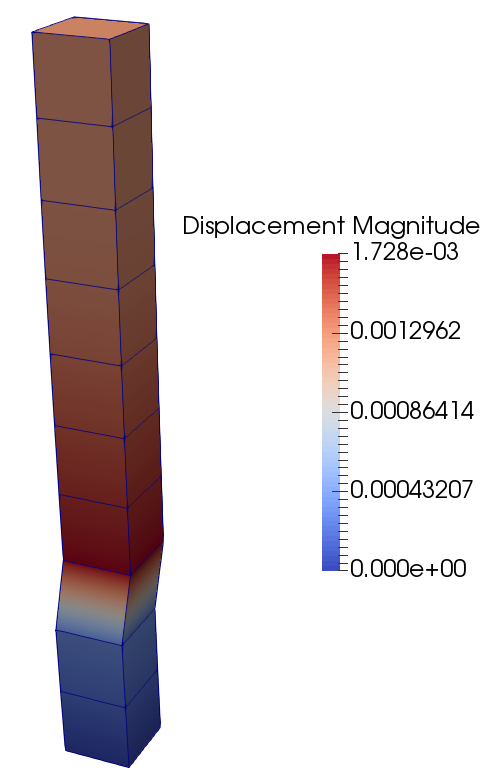
\includegraphics[width = 6cm]{./Figure-files/nonlinear_analysis_steps/free_field_1D/DRM1D_Motion3D.png}
  \caption{Simulation Model}
  \label{fig_decon_3D_motion_1D_model_results}
\end{figure}


The time series of simulation results is shown in Fig.~\ref{fig_decon_3D_motion_1D_model_results_top_bottom_time_series}.
\begin{figure}[H]
  \centering
  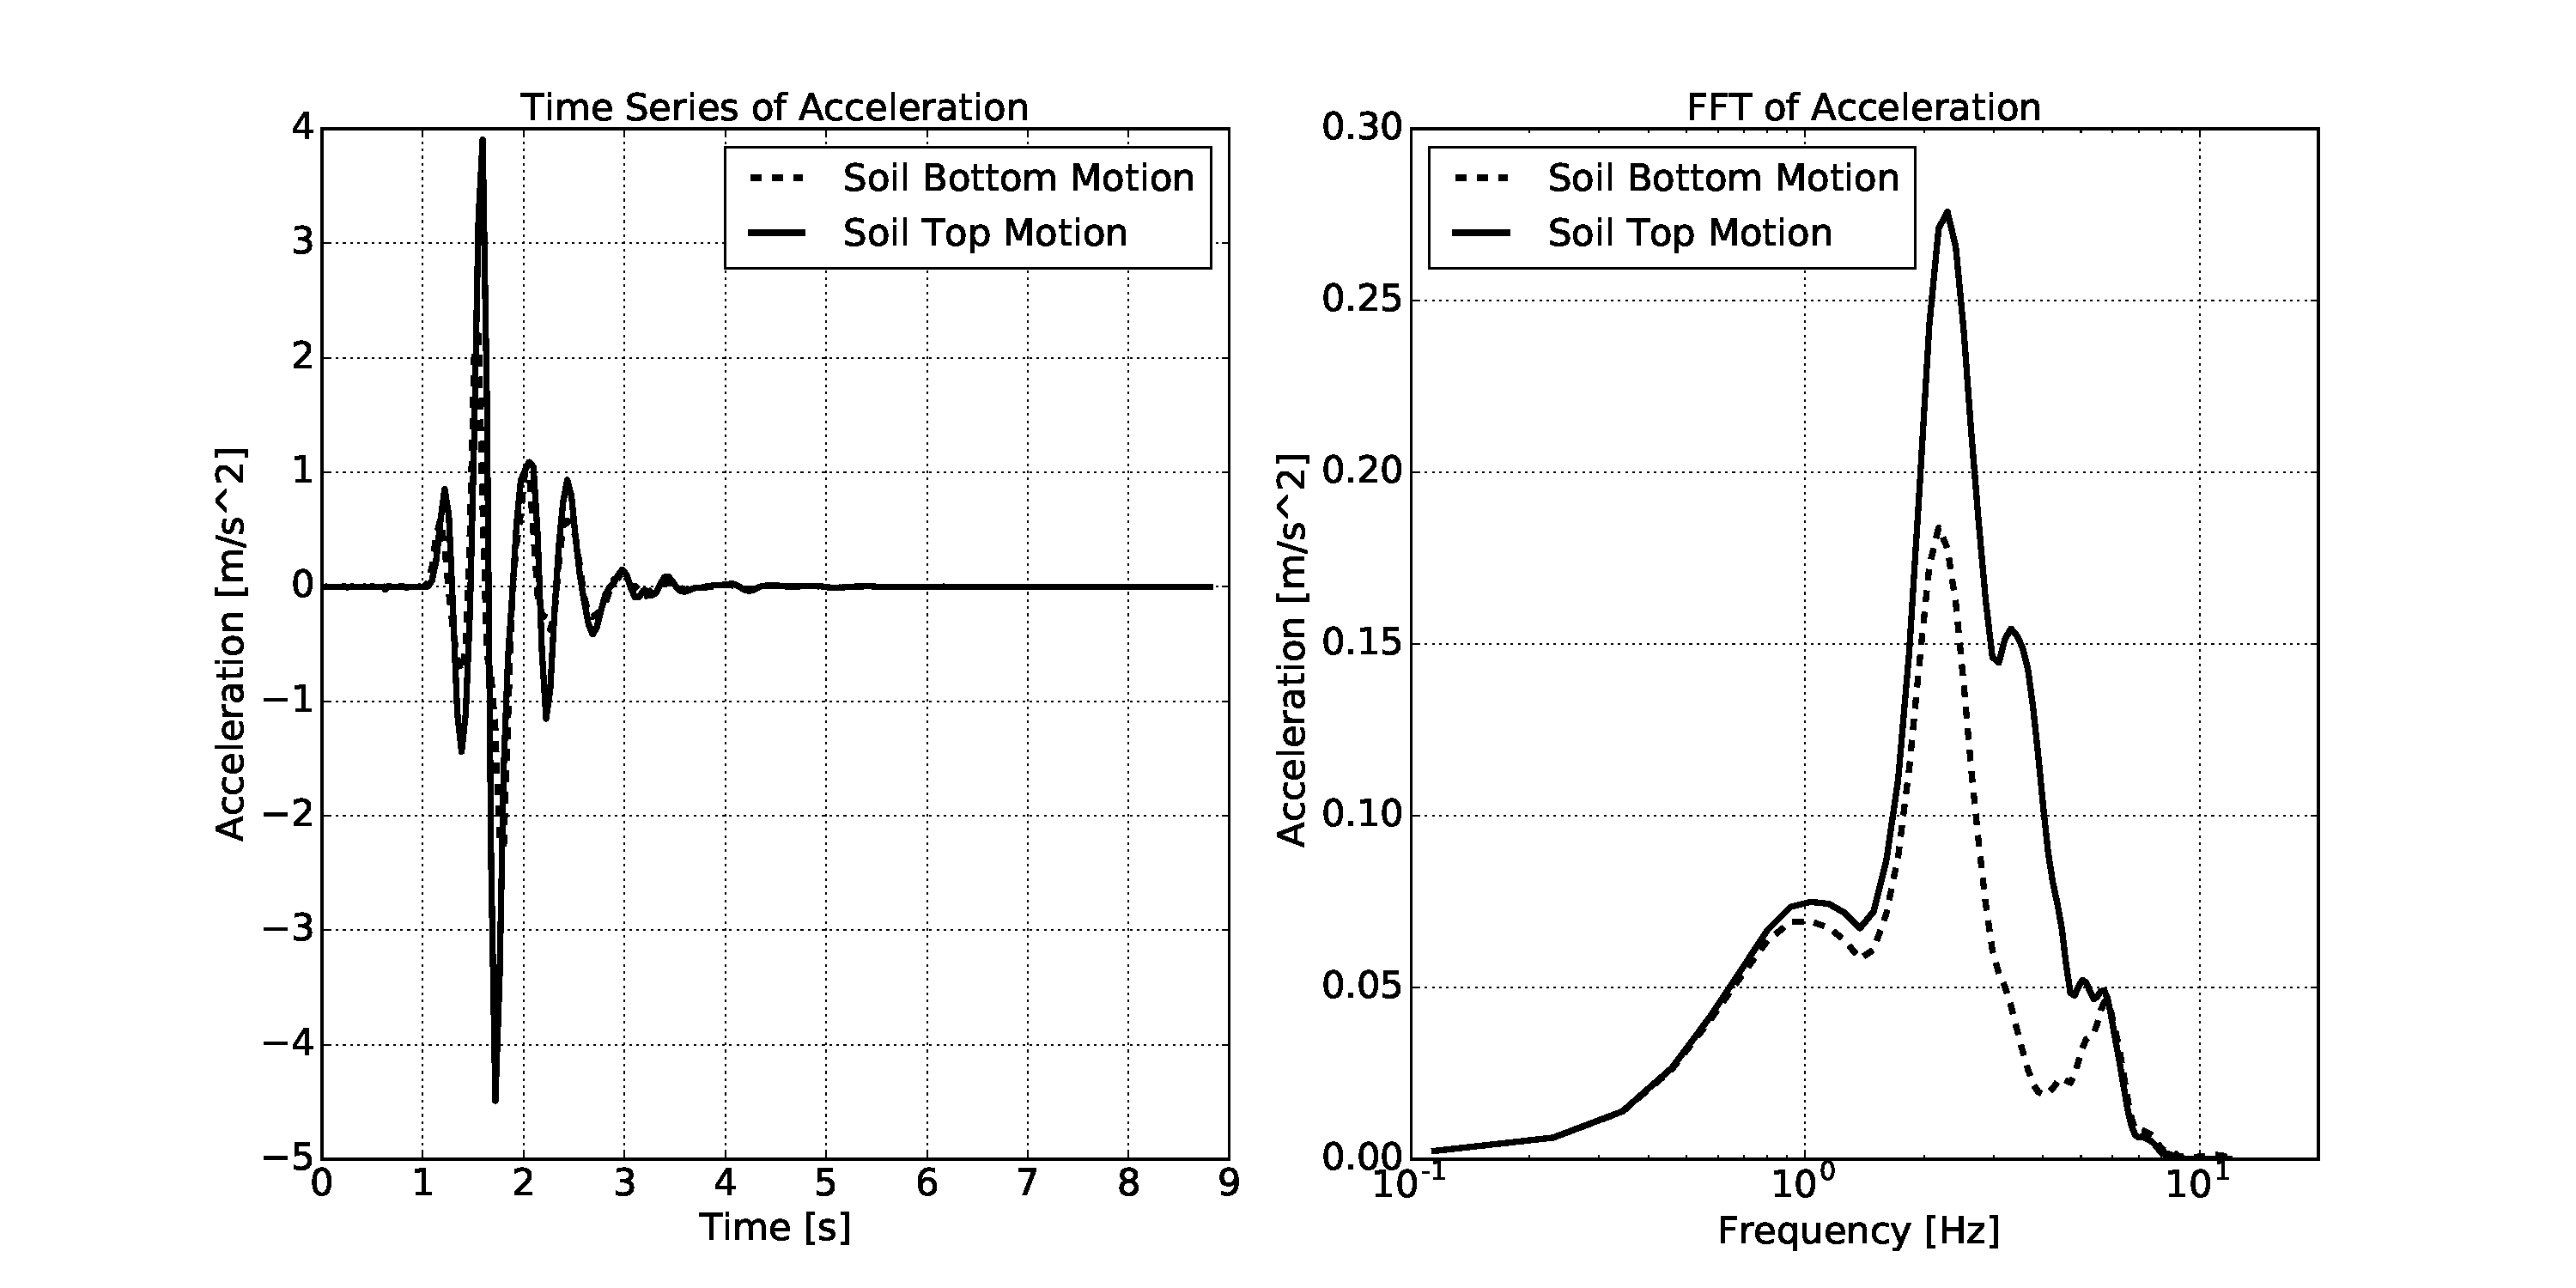
\includegraphics[width = 15cm]{./Figure-files/nonlinear_analysis_steps/free_field_1D/DRM1D_motion_node_5_x_acce_compare.pdf}
  \caption{Simulation Model}
  \label{fig_decon_3D_motion_1D_model_results_top_bottom_time_series}
\end{figure}

The response spectrum of motion is shown in Fig.~\ref{fig_spectrum_freq_period_time_series}.
\begin{figure}[H]
  \centering
  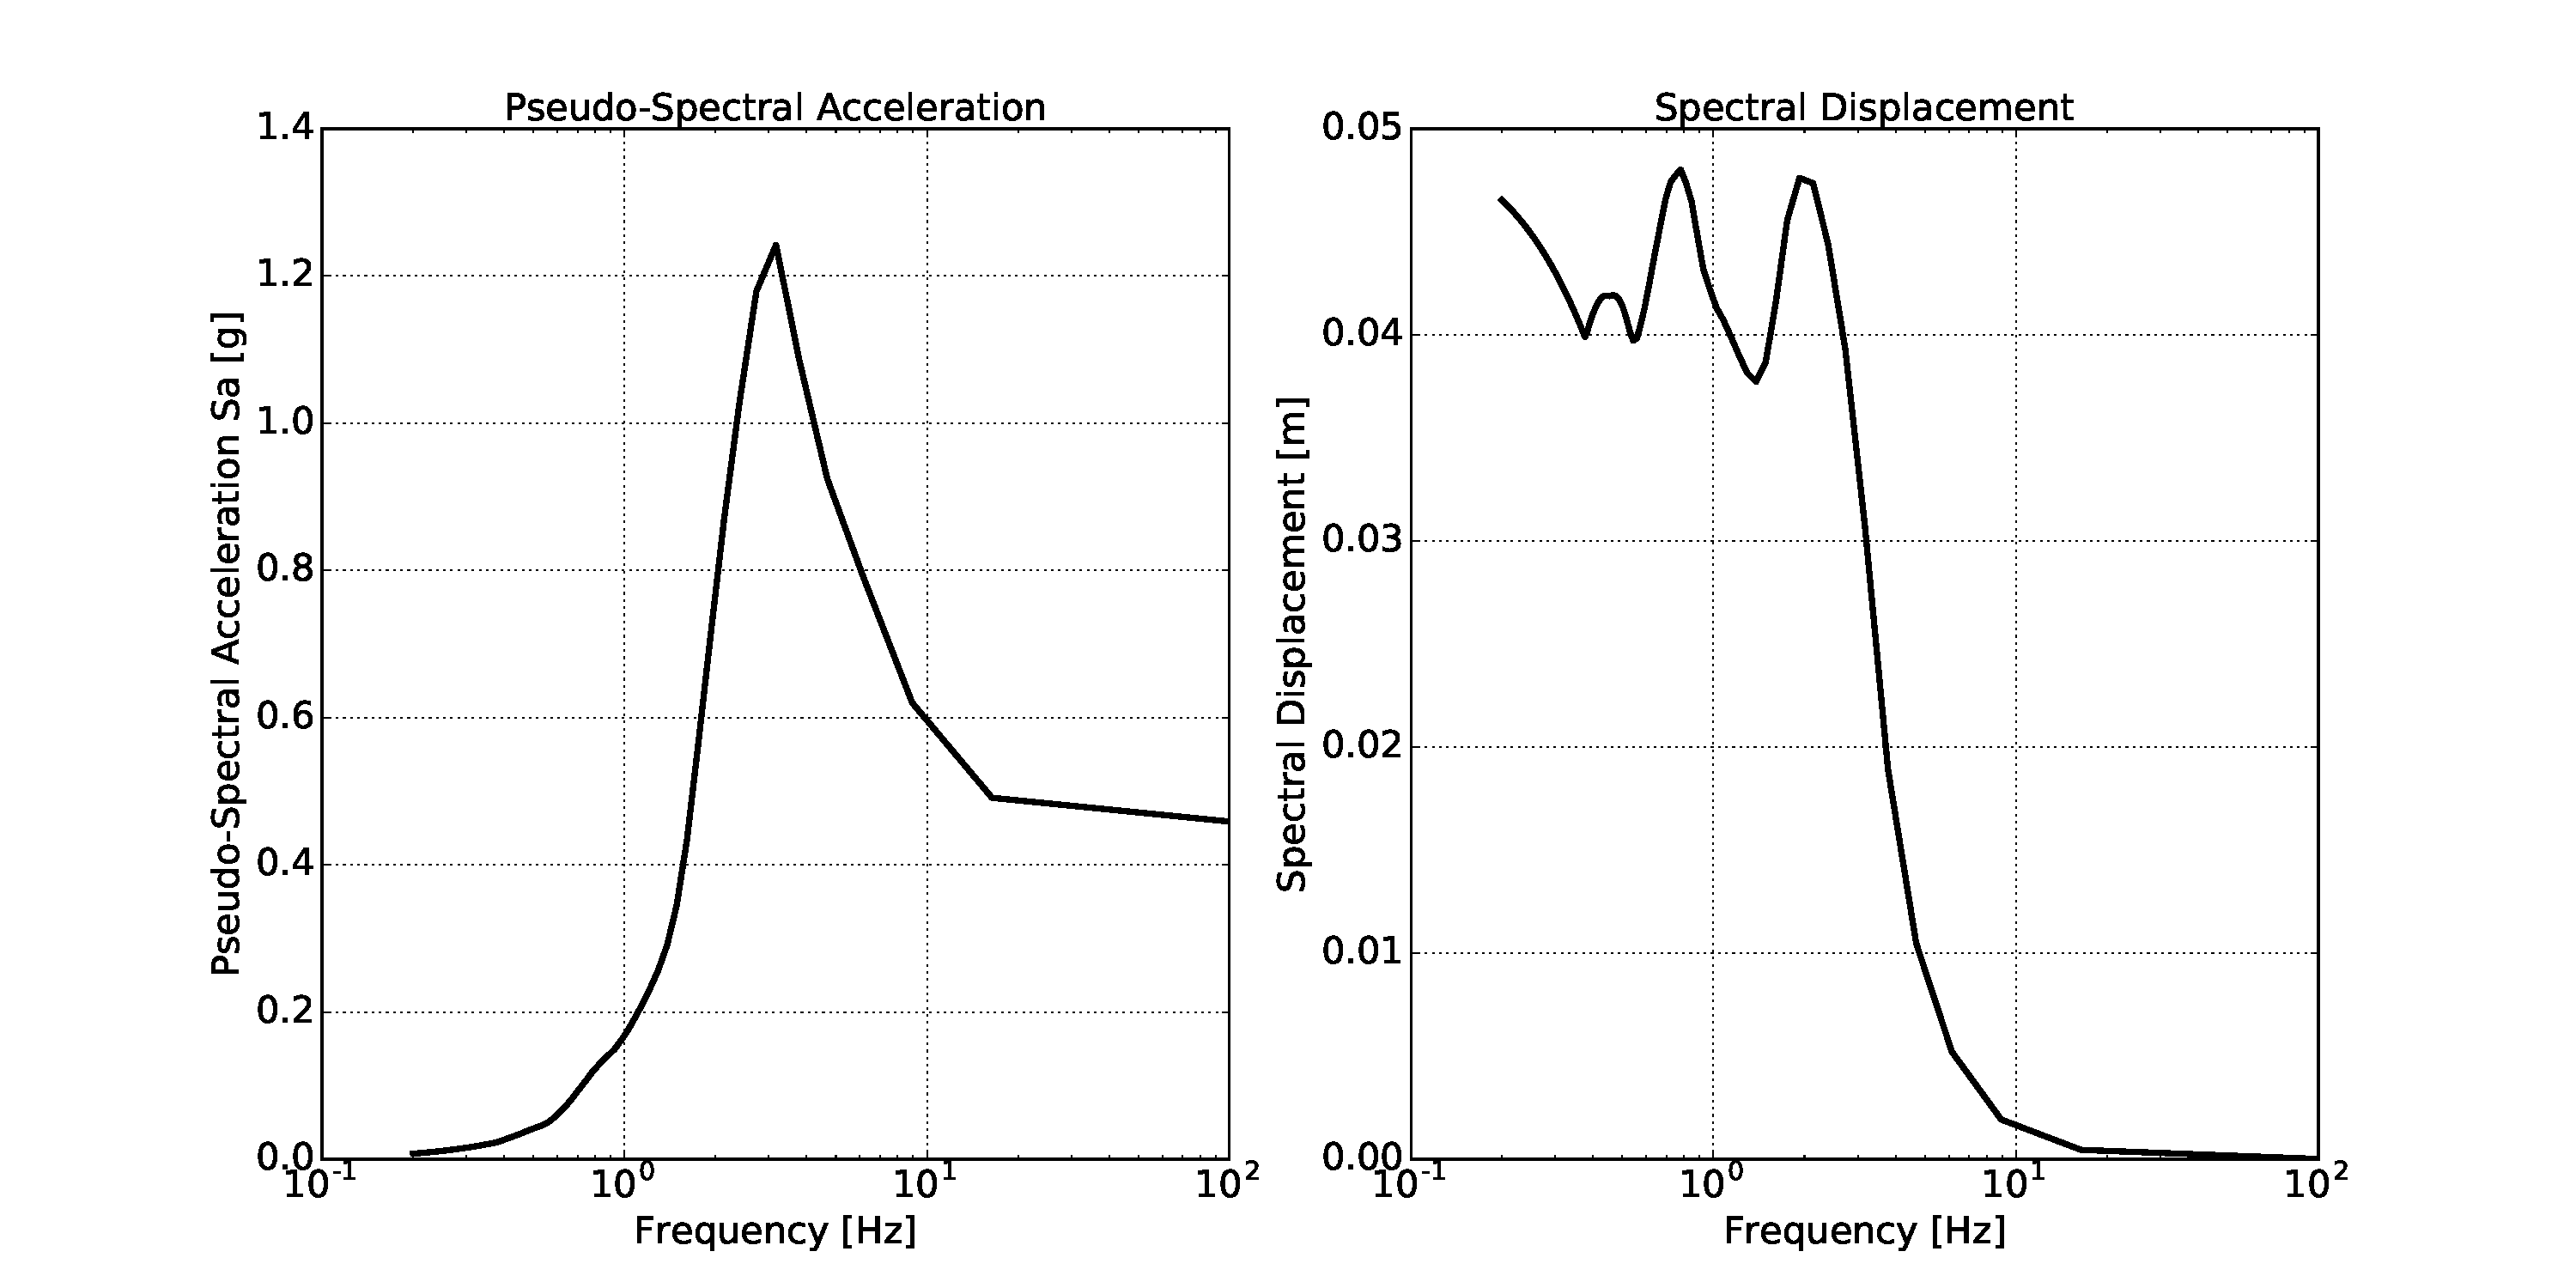
\includegraphics[width = 15cm]{./Figure-files/nonlinear_analysis_steps/free_field_1D/DRM1D_motion_node_5_x_spectrum_freq.pdf}
  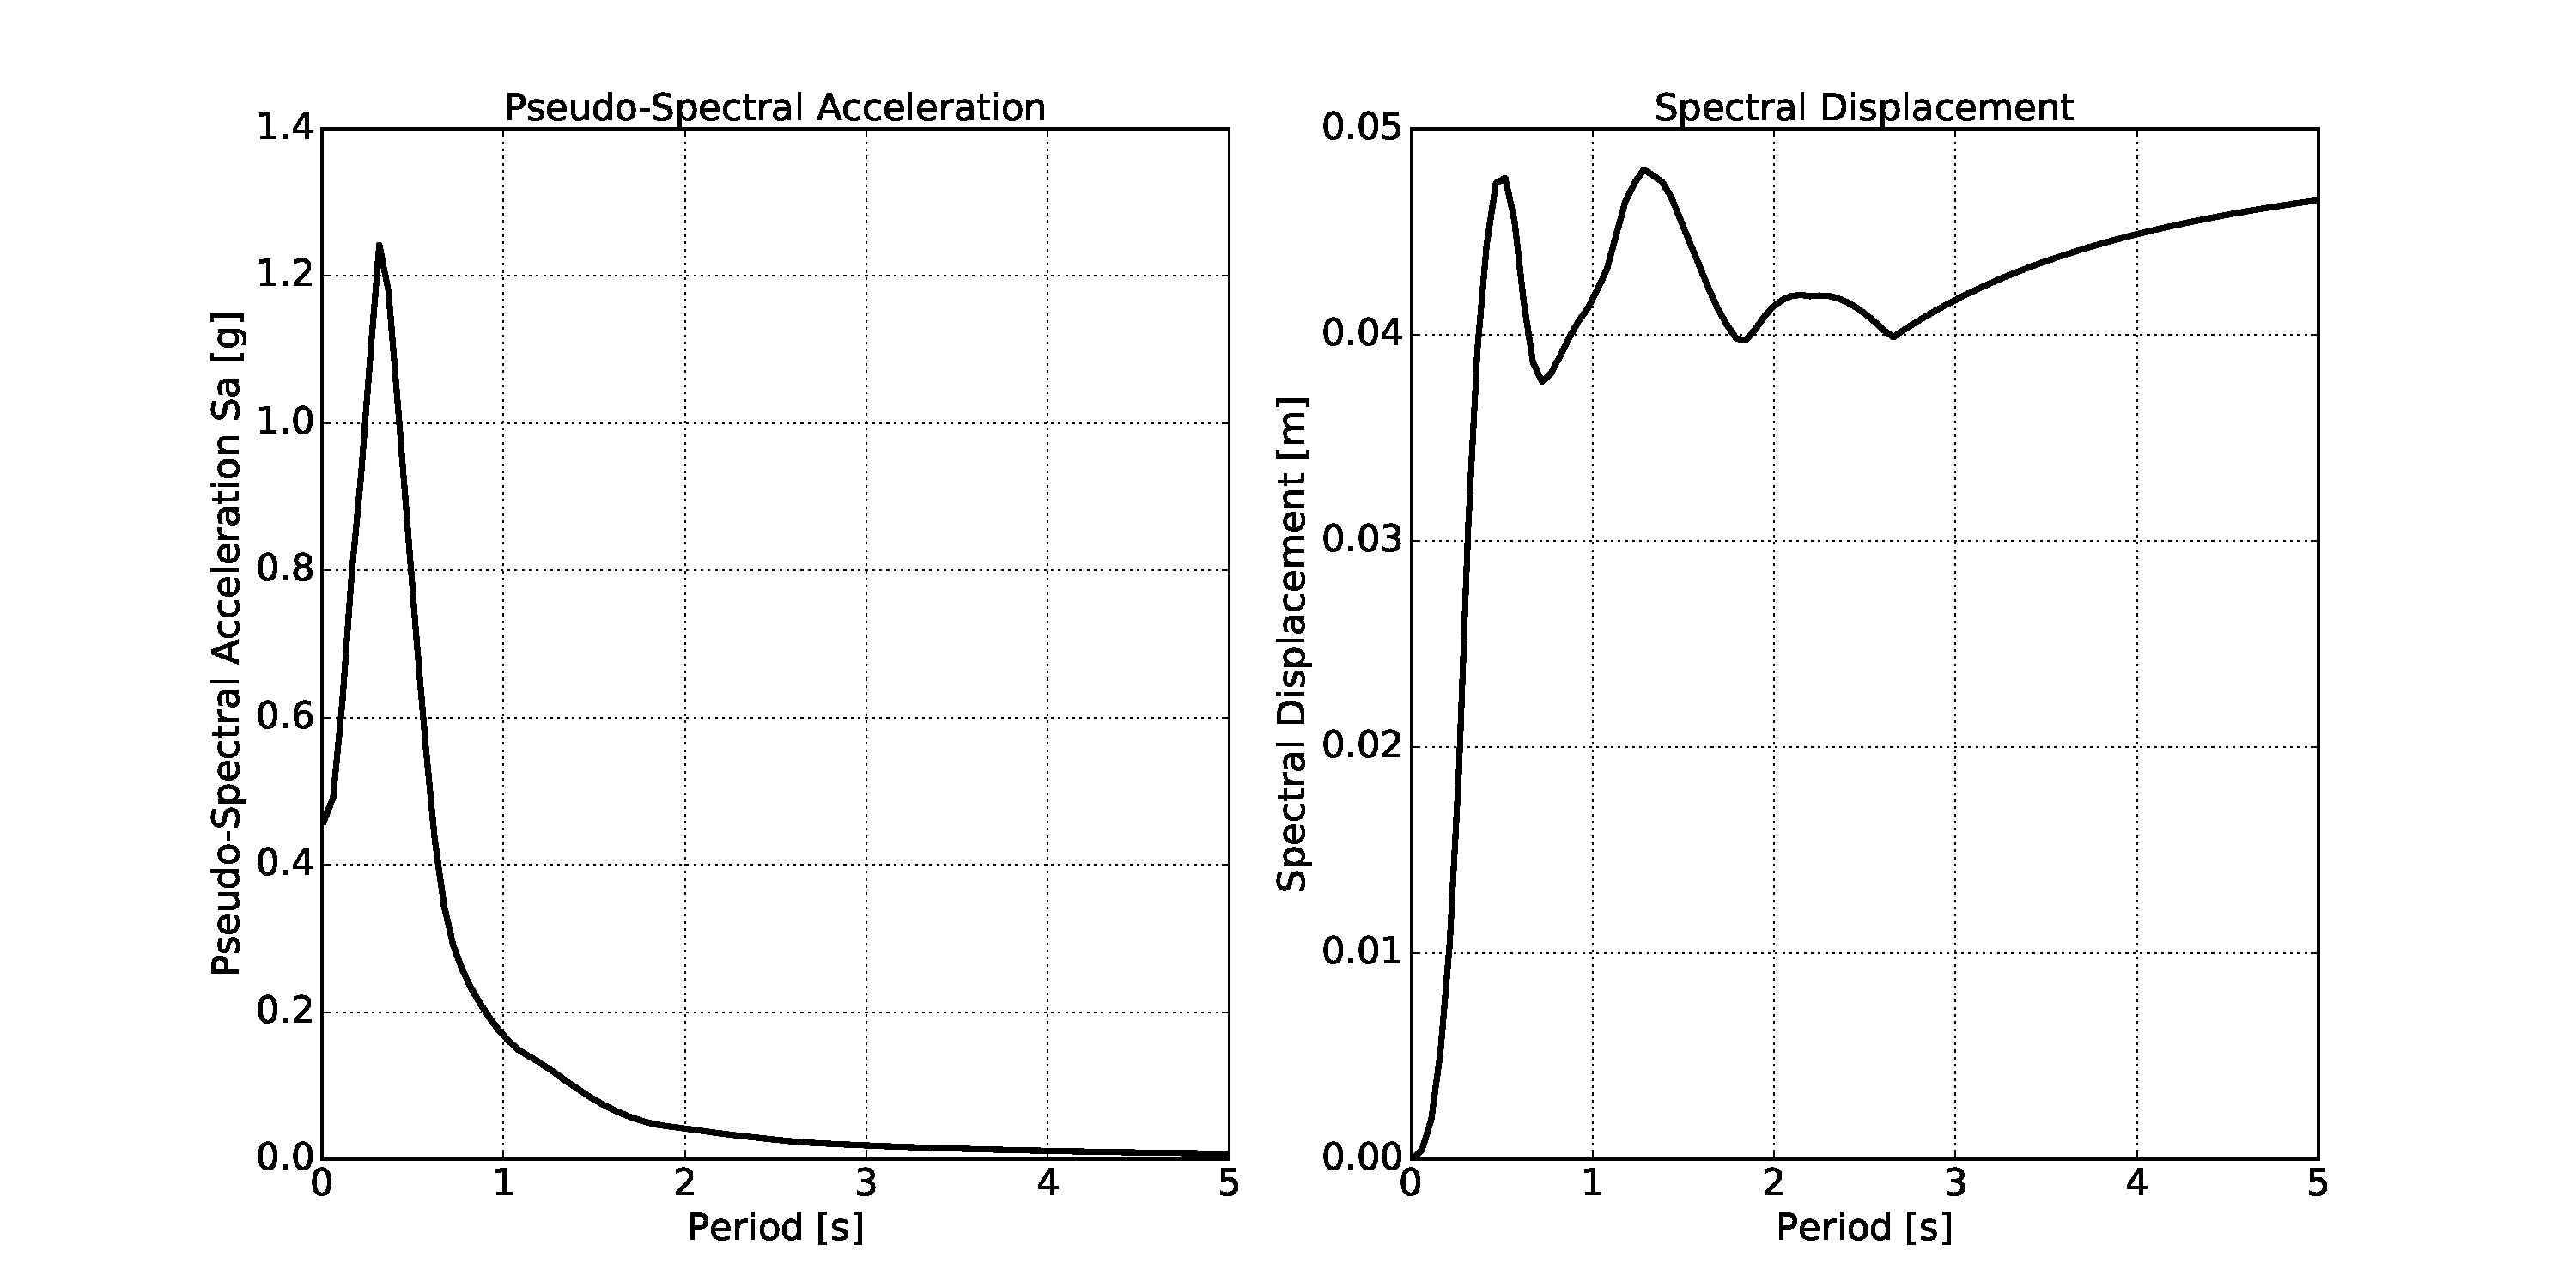
\includegraphics[width = 15cm]{./Figure-files/nonlinear_analysis_steps/free_field_1D/DRM1D_motion_node_5_x_spectrum_period.pdf}
  \caption{Simulation Model}
  \label{fig_spectrum_freq_period_time_series}
\end{figure}

% ******************************************************************
% ******************************************************************
% ******************************************************************
\clearpage
\newpage
\section{Free Field 3D}
\label{free_field_3D}

\paragraph{Elastic Material}
% The Real-ESSI input files for this example are available 
% \href{https://github.com/yuan-energy/Real-ESSI-Short-Course-Examples/tree/master/short-course-examples/nonlinear_analysis_steps/free_field_3D/elastic}{HERE}. 
The compressed package of input files is  
\href{https://github.com/yuan-energy/Real-ESSI-Short-Course-Examples/tree/master/short-course-examples/nonlinear_analysis_steps/free_field_3D/elastic/elastic.tgz?raw=true}{HERE}. 


The Modeling parameters are listed.
\begin{itemize}
  \item Elastic Material Properties 
  \begin{itemize}
    \item Mass density, $\rho$, \enspace \enspace 2000 $kg/m^3$
    \item Young's modulus, $E$, \enspace \enspace 1.1 GPa
    \item Poisson's ratio, $\nu$, \enspace \enspace 0.1
  \end{itemize}
\end{itemize}


SIMULATION TIME: With 8 cores on AWS EC2 c4.2xlarge instance, the running time for this example is 5 minutes.

\paragraph{von-Mises Armstrong-Frederick Material}
% The Real-ESSI input files for this example are available 
% \href{https://github.com/yuan-energy/Real-ESSI-Short-Course-Examples/tree/master/short-course-examples/nonlinear_analysis_steps/free_field_3D/elastoplastic}{HERE}. 
The compressed package of input files is  
\href{https://github.com/yuan-energy/Real-ESSI-Short-Course-Examples/tree/master/short-course-examples/nonlinear_analysis_steps/free_field_3D/elastoplastic/elastoplastic.tgz?raw=true}{HERE}. 

The Modeling parameters are listed.
\begin{itemize}
  \item von-Mises nonlinear hardening material model 
  \begin{itemize}
    \item Mass density, $\rho$, \enspace \enspace 2000 $kg/m^3$
    \item Young's modulus, $E$, \enspace \enspace 1.1 GPa
    \item Poisson's ratio, $\nu$, \enspace \enspace 0.1
    \item von Mises radius, $k$, \enspace \enspace 60 kPa
    \item nonlinear kinematic hardening rate, $H_a$, \enspace \enspace  30 MPa
    \item nonlinear kinematic hardening rate, $C_r$, \enspace \enspace  25
    \item isotropic hardening rate, $K_{iso}$, \enspace \enspace 0 Pa
  \end{itemize}
\end{itemize}

SIMULATION TIME: With 8 cores on AWS EC2 c4.2xlarge instance, the running time for this example is 17 minutes.

\paragraph{von-Mises G/Gmax Material}
% The Real-ESSI input files for vonMisesGoverGmax material example are available 
% \href{https://github.com/yuan-energy/Real-ESSI-Short-Course-Examples/tree/master/short-course-examples/nonlinear_analysis_steps/free_field_3D/vonMisesGoverGmax}{HERE}. 
The compressed package of input files is  
\href{https://github.com/yuan-energy/Real-ESSI-Short-Course-Examples/tree/master/short-course-examples/nonlinear_analysis_steps/free_field_3D/vonMisesGoverGmax/vonMisesGoverGmax.tgz?raw=true}{HERE}. 

The Modeling parameters are listed.
\begin{itemize}
  \item von-Mises G/Gmax material model 
  \begin{itemize}
    \item Mass density, $\rho$, \enspace \enspace 2000 $kg/m^3$
    \item Young's modulus, $E$, \enspace \enspace 1.1 GPa
    \item Poisson's ratio, $\nu$, \enspace \enspace 0.1
    \item Total number of shear modulus \enspace \enspace  9
    \item G over Gmax, \enspace \enspace  1,0.995,0.966,0.873,0.787,0.467,0.320,0.109,0.063
    \item Shear strain gamma, \enspace \enspace  0,1E-6,1E-5,5E-5,1E-4, 0.0005, 0.001, 0.005, 0.01
  \end{itemize}
\end{itemize}


SIMULATION TIME: With 8 cores on AWS EC2 c4.2xlarge instance, the running time for this example is 565 minutes.

\paragraph{Drucker-Prager G/Gmax Material}
% The Real-ESSI input files for this example are available 
% \href{https://github.com/yuan-energy/Real-ESSI-Short-Course-Examples/tree/master/short-course-examples/nonlinear_analysis_steps/free_field_3D/DruckerPragerGoverGmax}{HERE}. 
The compressed package of input files is  
\href{https://github.com/yuan-energy/Real-ESSI-Short-Course-Examples/tree/master/short-course-examples/nonlinear_analysis_steps/free_field_3D/DruckerPragerGoverGmax/DruckerPragerGoverGmax.tgz?raw=true}{HERE}. 

The Modeling parameters are listed.
\begin{itemize}
  \item Drucker-Prager G/Gmax material model 
  \begin{itemize}
    \item Mass density, $\rho$, \enspace \enspace 2000 $kg/m^3$
    \item Young's modulus, $E$, \enspace \enspace 1.1 GPa
    \item Poisson's ratio, $\nu$, \enspace \enspace 0.1
    \item Initial confining stress, $p_0$, \enspace \enspace 100 kPa
    \item Reference pressure, $p_{refer} $, \enspace \enspace 100 kPa
    \item Pressure exponential, $ n  $, \enspace \enspace 0.5
    \item Cohesion, $ n  $, \enspace \enspace 1 kPa
    \item Total number of Shear Modulus \enspace \enspace 9
    \item G over Gmax, \enspace \enspace  1,0.995,0.966,0.873,0.787,0.467,0.320,0.109,0.063
    \item Shear strain gamma, \enspace \enspace  0,1E-6,1E-5,5E-5,1E-4, 0.0005, 0.001, 0.005, 0.01
  \end{itemize}
\end{itemize}


SIMULATION TIME: With 8 cores on AWS EC2 c4.2xlarge instance, the running time for this example is 565 minutes.




\begin{figure}[H]
  \centering
  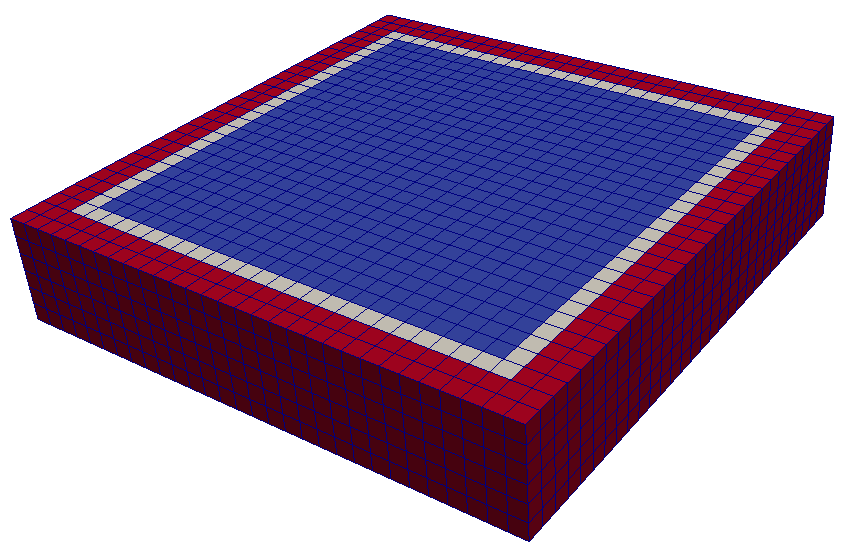
\includegraphics[width = 8cm]{./Figure-files/nonlinear_analysis_steps/free_field_3D/overview.png}
  \caption{Simulation Model}
  \label{fig_nonlinear_motion_3D_model}
\end{figure}

The illustration results of the simulation is shown in Fig.~\ref{fig_decon_3D_motion_3D_model_results_free_field}.
As shown in the results, outside the DRM layer, there is no outgoing waves. 

\begin{figure}[H]
  \centering
  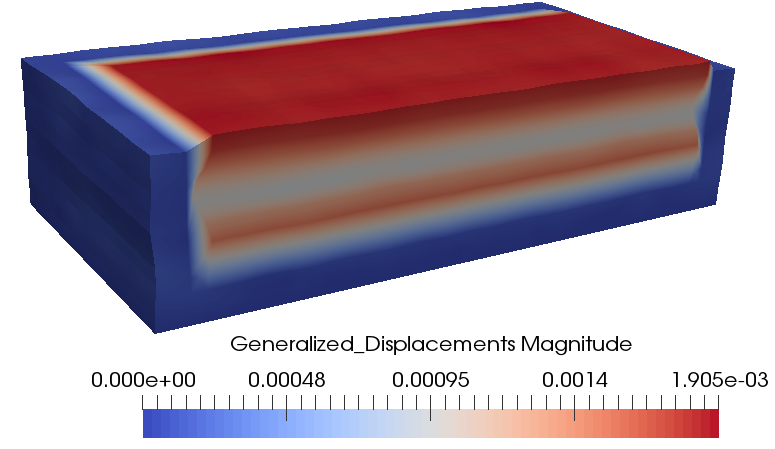
\includegraphics[width = 10cm]{./Figure-files/nonlinear_analysis_steps/free_field_3D/motion3D_DRM3D_free_field.png}
  \caption{Simulation Model}
  \label{fig_nonlinear_steps_D_motion_3D_model_results_free_field}
\end{figure}


The node tags of critical points for postprocessing are shown in Fig.\ref{fig_points_soil_foundation}.

\begin{figure}[H]
  \centering
  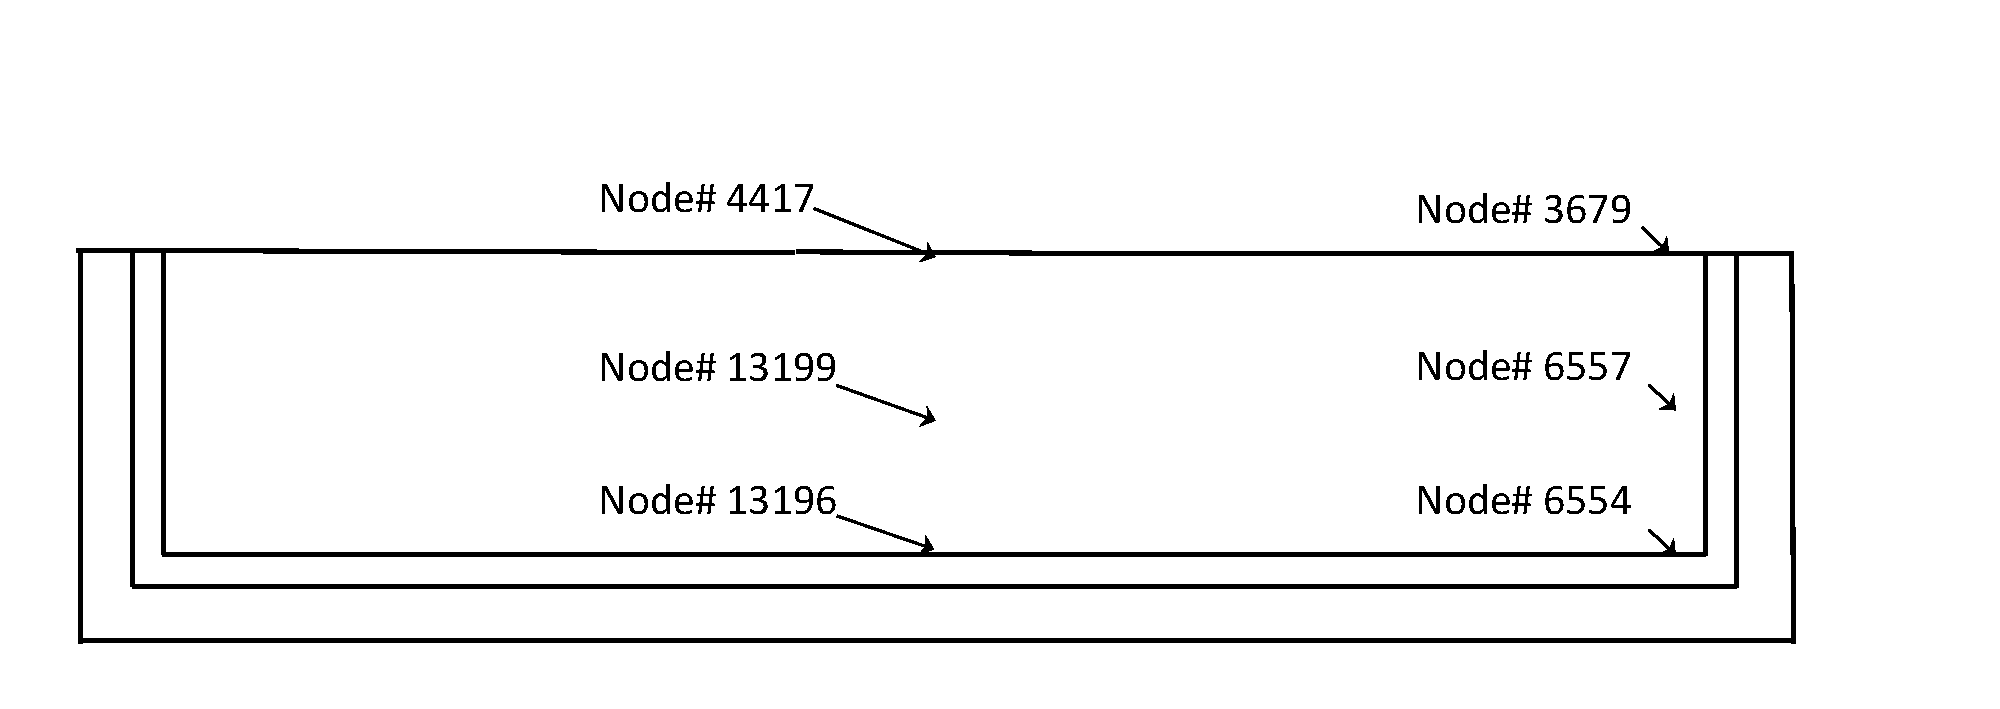
\includegraphics[width = 12cm]{./Figure-files/nonlinear_analysis_steps/free_field_3D/free_field_3D_node_location.pdf}
  \caption{Critical Points of Simulation Model}
  \label{fig_points_soil_foundation}
\end{figure}

SIMULATION TIME: With 8 cores on AWS EC2 c4.2xlarge instance, the running time for this example is 871 minutes.


The time series of simulation results is shown in Fig.~\ref{fig_decon_3D_motion_1D_model_results_top_bottom_time_series_fr3d}.
\begin{figure}[H]
  \centering
  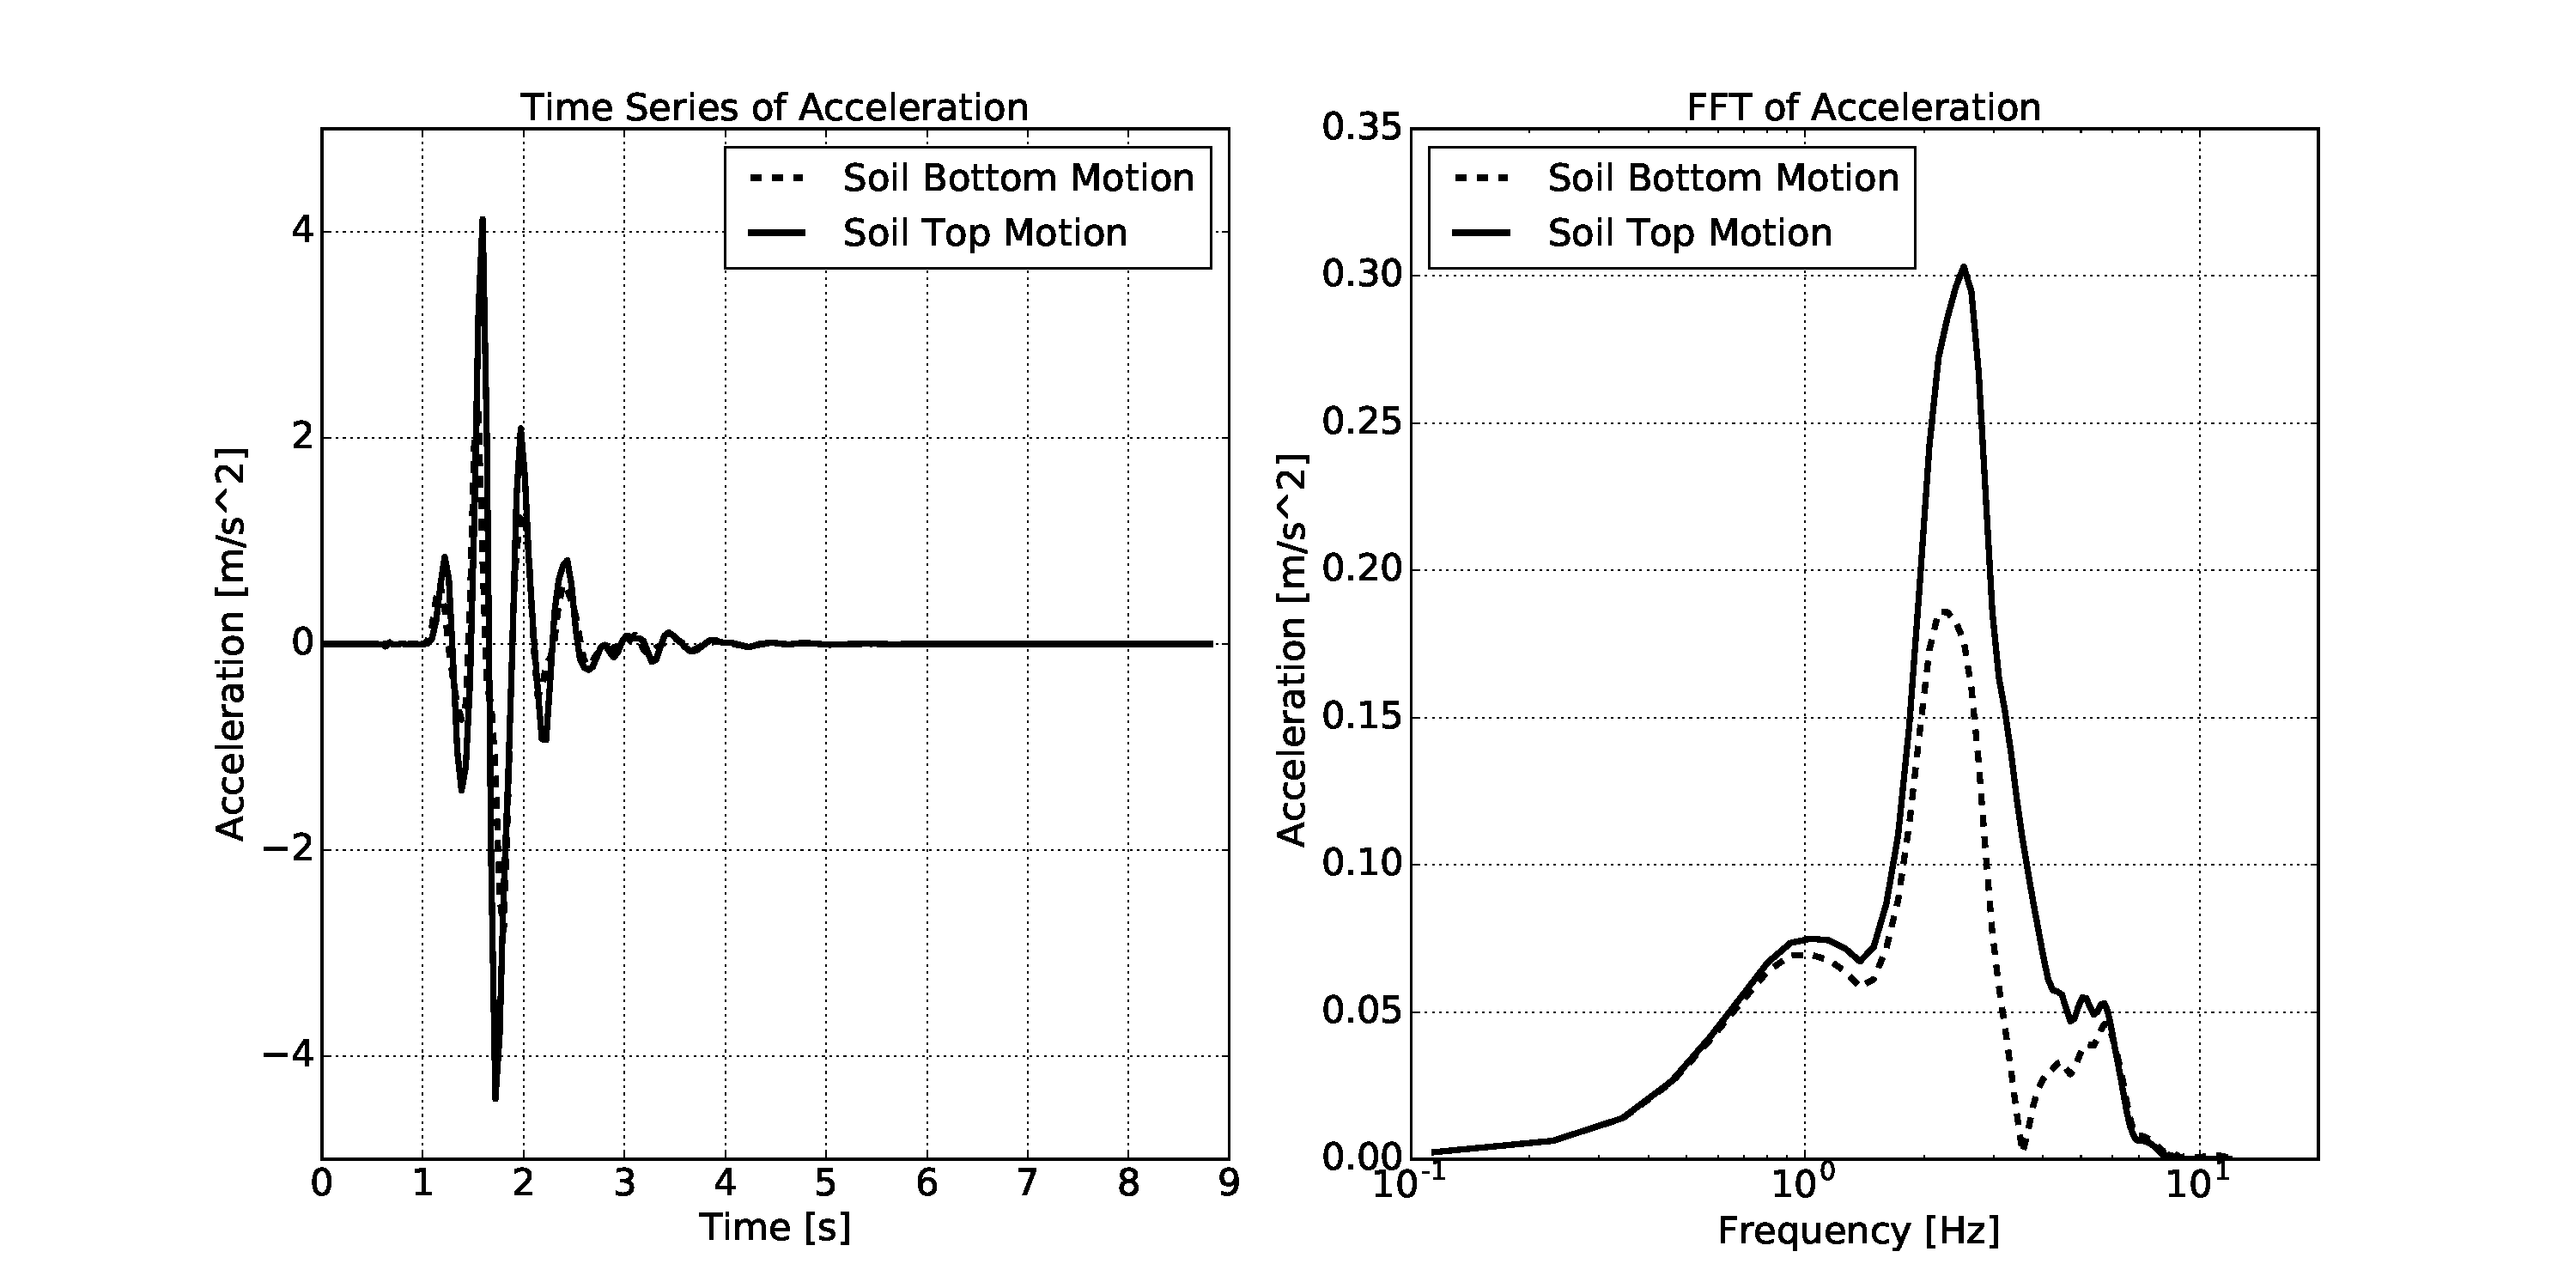
\includegraphics[width = 15cm]{./Figure-files/nonlinear_analysis_steps/free_field_3D/DRM3D_motion_node_4454_x_acce_compare.pdf}
  \caption{Simulation Model}
  \label{fig_decon_3D_motion_1D_model_results_top_bottom_time_series_fr3d}
\end{figure}

The response spectrum of motion is shown in Fig.~\ref{fig_spectrum_freq_period_time_series_fr3d}.
\begin{figure}[H]
  \centering
  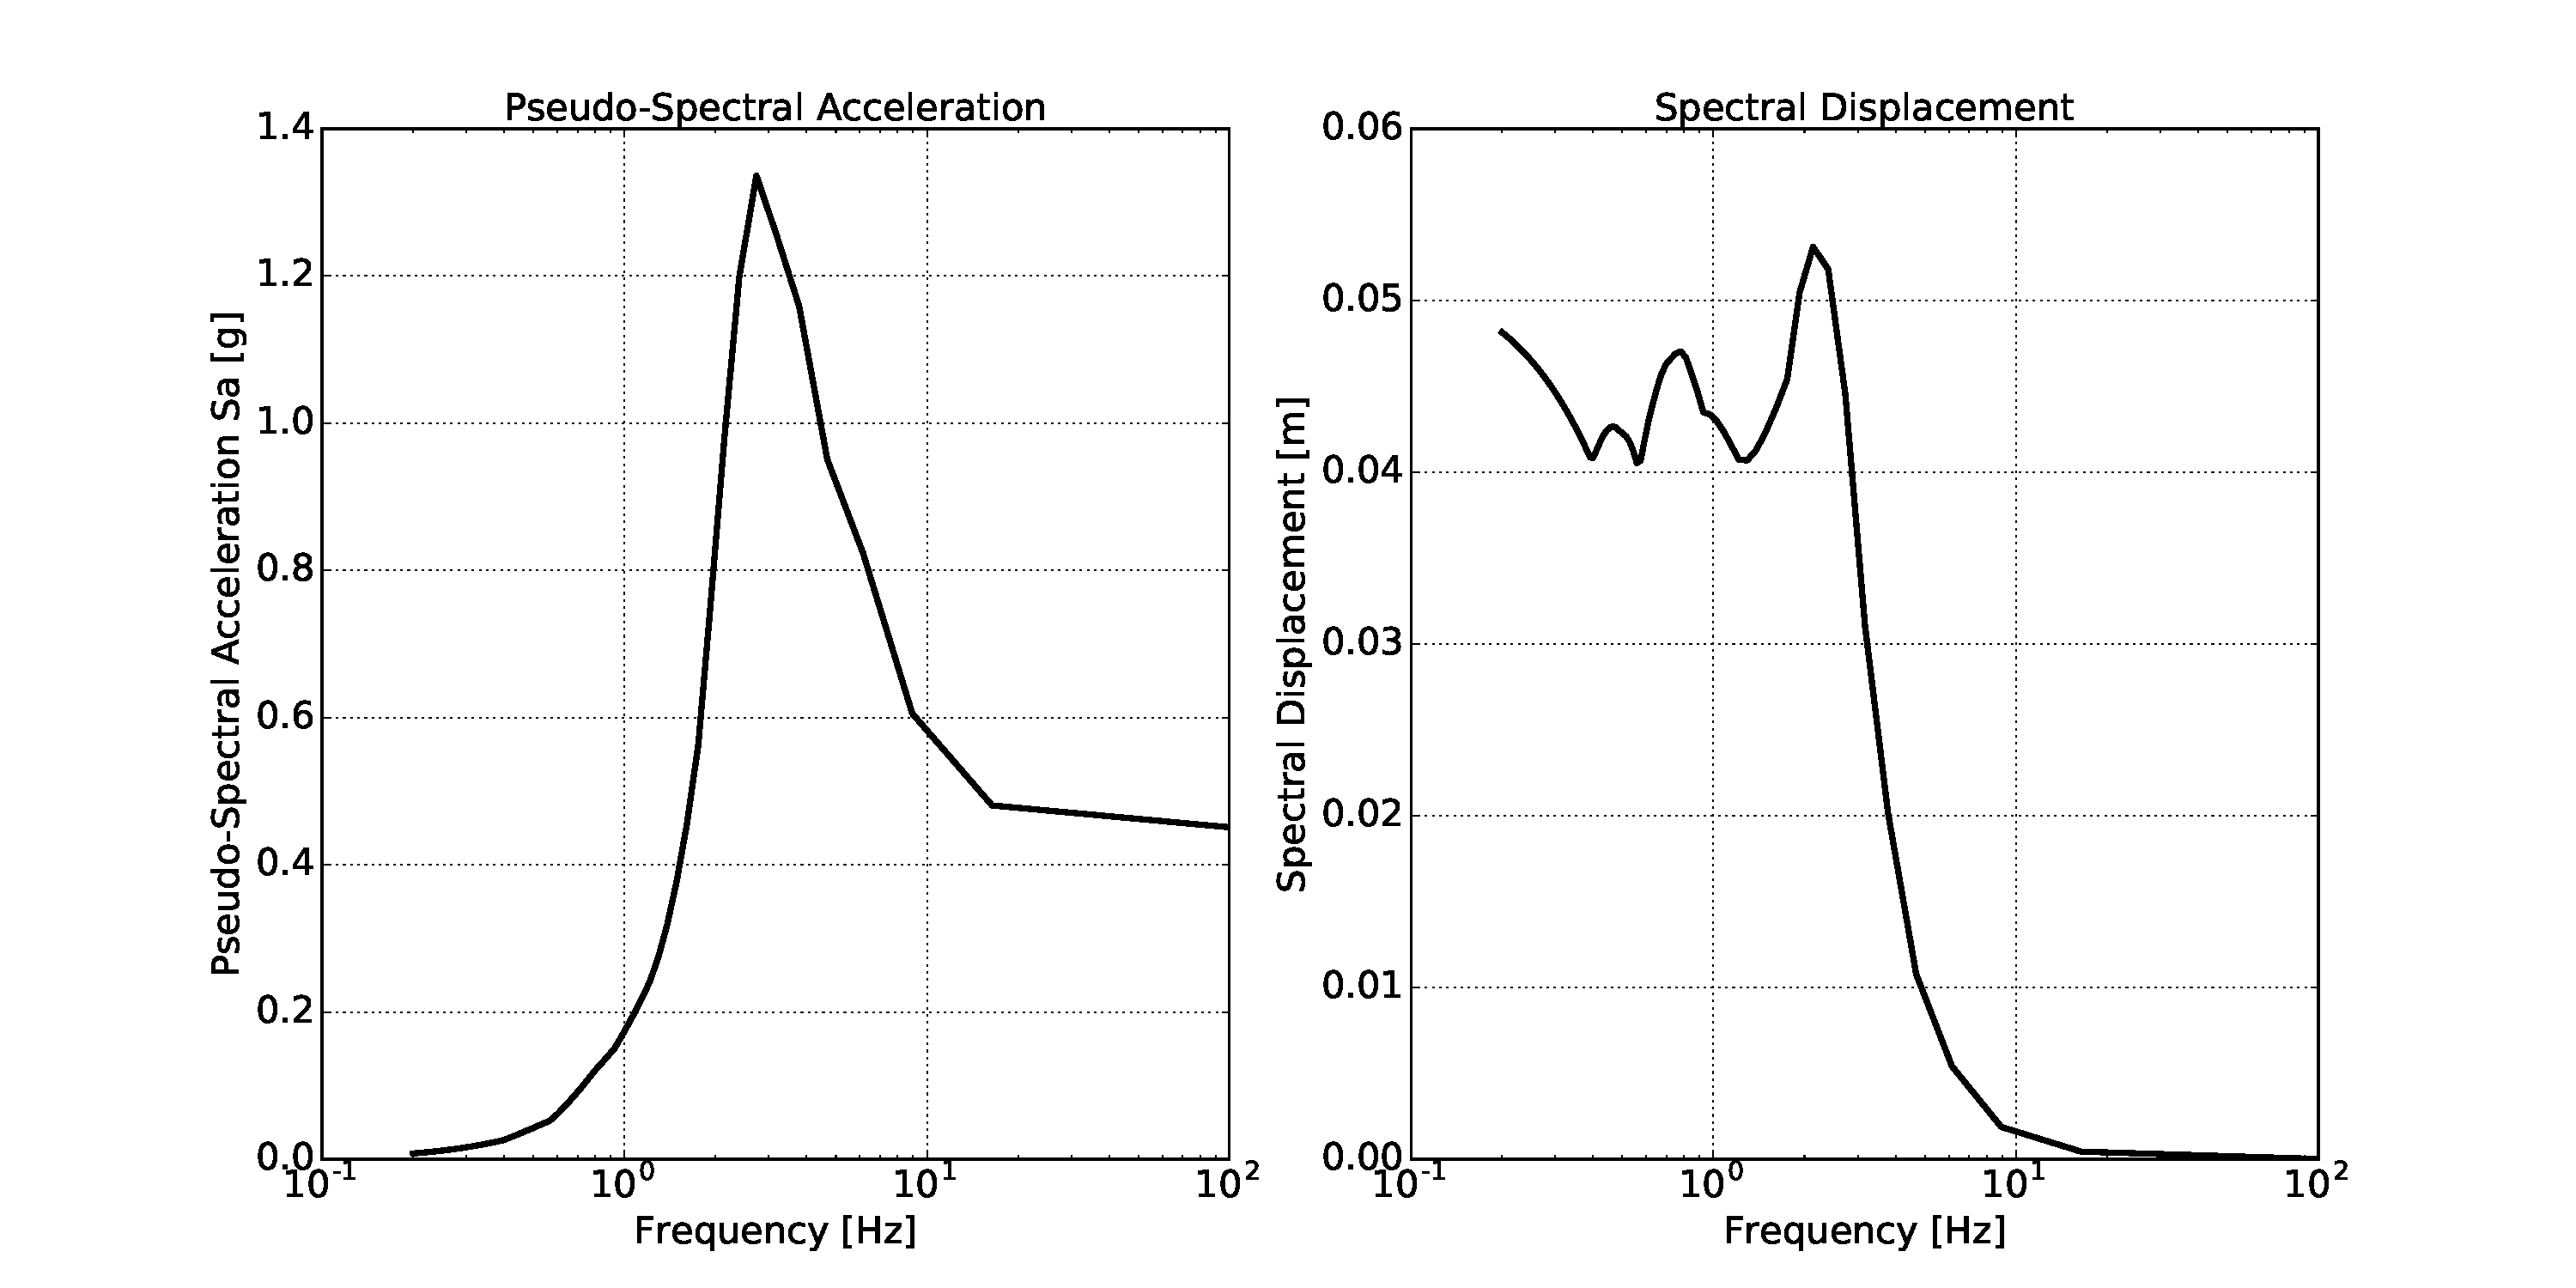
\includegraphics[width = 15cm]{./Figure-files/nonlinear_analysis_steps/free_field_3D/DRM3D_motion_node_4454_x_spectrum_freq.pdf}
  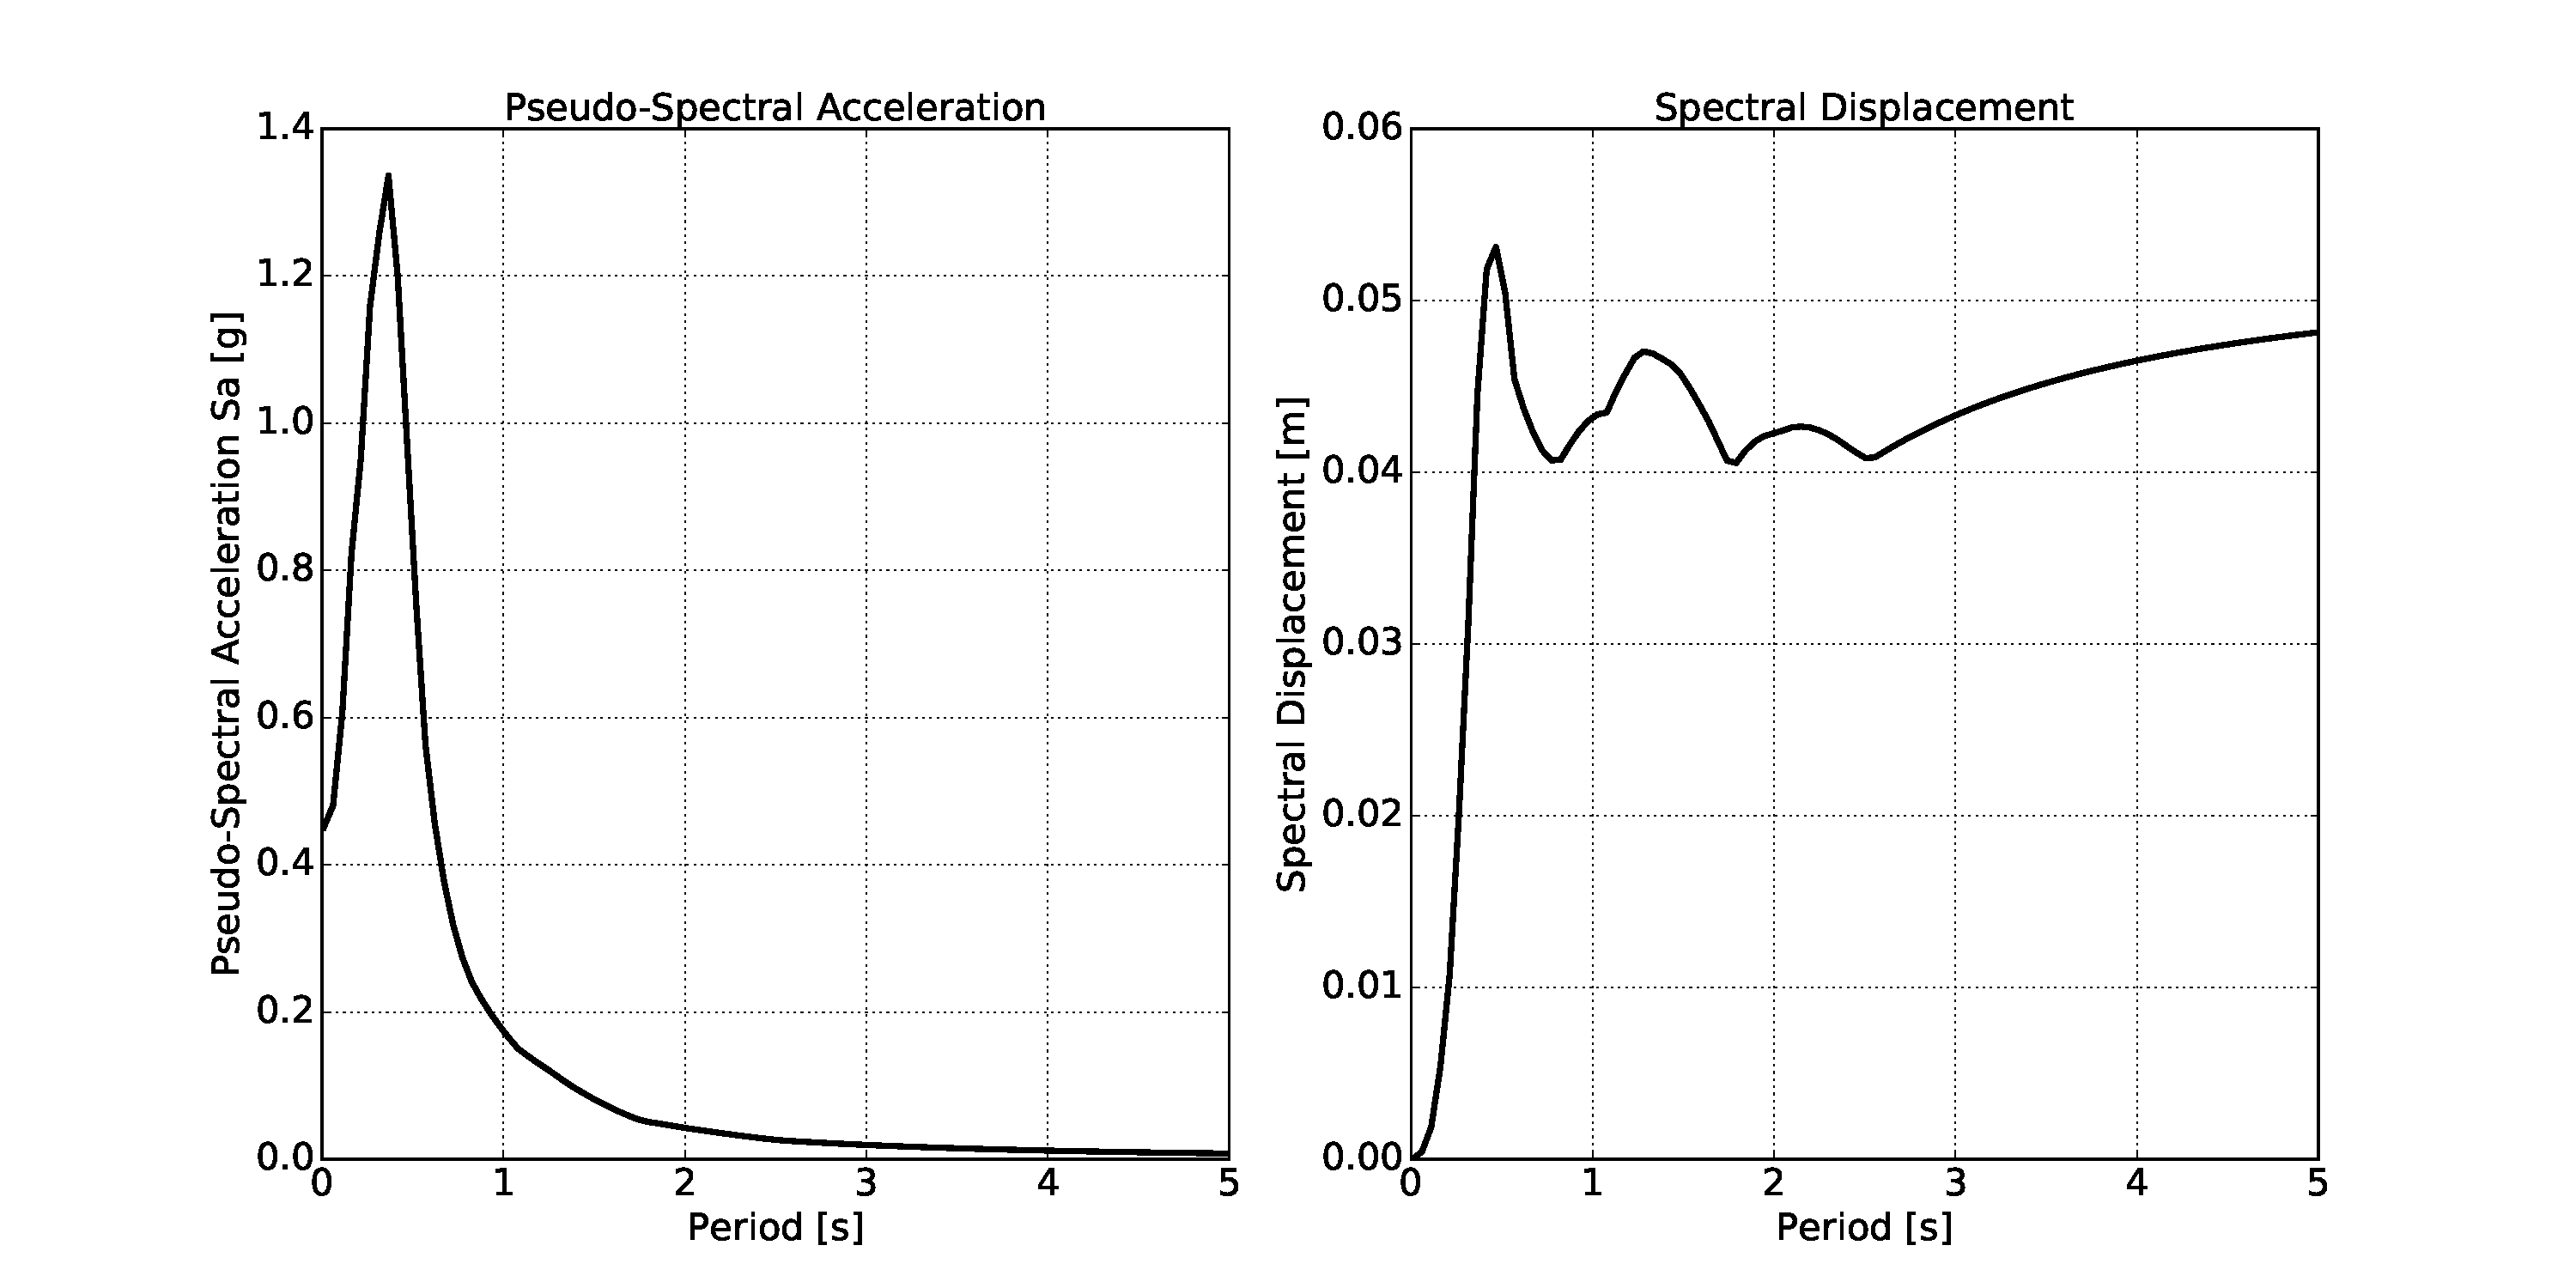
\includegraphics[width = 15cm]{./Figure-files/nonlinear_analysis_steps/free_field_3D/DRM3D_motion_node_4454_x_spectrum_period.pdf}
  \caption{Simulation Model}
  \label{fig_spectrum_freq_period_time_series_fr3d}
\end{figure}


% ******************************************************************
% ******************************************************************
% ******************************************************************
\clearpage
\newpage
\section{Soil-Foundation Interaction 3D}
\label{foundation_3D}


\paragraph{Elastic Material}
% The Real-ESSI input files for this example are available 
% \href{https://github.com/yuan-energy/Real-ESSI-Short-Course-Examples/tree/master/short-course-examples/nonlinear_analysis_steps/soil-foundation/elastic}{HERE}. 
The compressed package of input files is  
\href{https://github.com/yuan-energy/Real-ESSI-Short-Course-Examples/tree/master/short-course-examples/nonlinear_analysis_steps/soil-foundation/elastic/elastic.tgz?raw=true}{HERE}. 

The Modeling parameters are listed.
\begin{itemize}
  \item Elastic Material Properties 
  \begin{itemize}
    \item Mass density, $\rho$, \enspace \enspace 2000 $kg/m^3$
    \item Young's modulus, $E$, \enspace \enspace 1.1 GPa
    \item Poisson's ratio, $\nu$, \enspace \enspace 0.1
  \end{itemize}
\end{itemize}

SIMULATION TIME: With 8 cores on AWS EC2 c4.2xlarge instance, the running time for this example is 13 minutes.

\paragraph{von-Mises Armstrong-Frederick Material}
% The Real-ESSI input files for this example are available 
% \href{https://github.com/yuan-energy/Real-ESSI-Short-Course-Examples/tree/master/short-course-examples/nonlinear_analysis_steps/soil-foundation/vonMisesArmstrongFrederick}{HERE}. 
The compressed package of input files is  
\href{https://github.com/yuan-energy/Real-ESSI-Short-Course-Examples/tree/master/short-course-examples/nonlinear_analysis_steps/soil-foundation/vonMisesArmstrongFrederick/vonMisesArmstrongFrederick.tgz?raw=true}{HERE}. 


The Modeling parameters are listed.
\begin{itemize}
  \item von-Mises nonlinear hardening material model 
  \begin{itemize}
    \item Mass density, $\rho$, \enspace \enspace 2000 $kg/m^3$
    \item Young's modulus, $E$, \enspace \enspace 1.1 GPa
    \item Poisson's ratio, $\nu$, \enspace \enspace 0.1
    \item von Mises radius, $k$, \enspace \enspace 60 kPa
    \item nonlinear kinematic hardening rate, $H_a$, \enspace \enspace  30 MPa
    \item nonlinear kinematic hardening rate, $C_r$, \enspace \enspace  25
    \item isotropic hardening rate, $K_{iso}$, \enspace \enspace 0 Pa
  \end{itemize}
\end{itemize}


SIMULATION TIME: With 8 cores on AWS EC2 c4.2xlarge instance, the running time for this example is 36 minutes.


\paragraph{von-Mises G/Gmax Material}
% The Real-ESSI input files for this example are available 
% \href{https://github.com/yuan-energy/Real-ESSI-Short-Course-Examples/tree/master/short-course-examples/nonlinear_analysis_steps/soil-foundation/vonMisesGoverGmax}{HERE}. 
The compressed package of input files is  
\href{https://github.com/yuan-energy/Real-ESSI-Short-Course-Examples/tree/master/short-course-examples/nonlinear_analysis_steps/soil-foundation/vonMisesGoverGmax/vonMisesGoverGmax.tgz?raw=true}{HERE}. 

The Modeling parameters are listed.
\begin{itemize}
  \item von-Mises G/Gmax material model 
  \begin{itemize}
    \item Mass density, $\rho$, \enspace \enspace 2000 $kg/m^3$
    \item Young's modulus, $E$, \enspace \enspace 1.1 GPa
    \item Poisson's ratio, $\nu$, \enspace \enspace 0.1
    \item Total number of shear modulus \enspace \enspace  9
    \item G over Gmax, \enspace \enspace  1,0.995,0.966,0.873,0.787,0.467,0.320,0.109,0.063
    \item Shear strain gamma, \enspace \enspace  0,1E-6,1E-5,5E-5,1E-4, 0.0005, 0.001, 0.005, 0.01
  \end{itemize}
\end{itemize}

SIMULATION TIME: With 8 cores on AWS EC2 c4.2xlarge instance, the running time for this example is 726 minutes.


\paragraph{Drucker-Prager G/Gmax Material}
% The Real-ESSI input files for this example are available 
% \href{https://github.com/yuan-energy/Real-ESSI-Short-Course-Examples/tree/master/short-course-examples/nonlinear_analysis_steps/soil-foundation/DruckerPragerGoverGmax}{HERE}. 
The compressed package of input files is  
\href{https://github.com/yuan-energy/Real-ESSI-Short-Course-Examples/tree/master/short-course-examples/nonlinear_analysis_steps/soil-foundation/DruckerPragerGoverGmax/DruckerPragerGoverGmax.tgz?raw=true}{HERE}. 


The Modeling parameters are listed.
\begin{itemize}
  \item Drucker-Prager G/Gmax material model 
  \begin{itemize}
    \item Mass density, $\rho$, \enspace \enspace 2000 $kg/m^3$
    \item Young's modulus, $E$, \enspace \enspace 1.1 GPa
    \item Poisson's ratio, $\nu$, \enspace \enspace 0.1
    \item Initial confining stress, $p_0$, \enspace \enspace 100 kPa
    \item Reference pressure, $p_{refer} $, \enspace \enspace 100 kPa
    \item Pressure exponential, $ n  $, \enspace \enspace 0.5
    \item Cohesion, $ n  $, \enspace \enspace 1 kPa
    \item Total number of Shear Modulus \enspace \enspace 9
    \item G over Gmax, \enspace \enspace  1,0.995,0.966,0.873,0.787,0.467,0.320,0.109,0.063
    \item Shear strain gamma, \enspace \enspace  0,1E-6,1E-5,5E-5,1E-4, 0.0005, 0.001, 0.005, 0.01
  \end{itemize}
\end{itemize}

SIMULATION TIME: With 8 cores on AWS EC2 c4.2xlarge instance, the running time for this example is 1252 minutes.


\paragraph{Contact Elements}
% The Real-ESSI input files for contact element example are available 
% \href{https://github.com/yuan-energy/Real-ESSI-Short-Course-Examples/tree/master/short-course-examples/nonlinear_analysis_steps/soil-foundation/contact}{HERE}. 
The compressed package of input files is  
\href{https://github.com/yuan-energy/Real-ESSI-Short-Course-Examples/tree/master/short-course-examples/nonlinear_analysis_steps/soil-foundation/contact/contact.tgz?raw=true}{HERE}. 


The Modeling parameters are listed.
\begin{itemize}
  \item Elastic Material Properties 
  \begin{itemize}
    \item Mass density, $\rho$, \enspace \enspace 2000 $kg/m^3$
    \item Young's modulus, $E$, \enspace \enspace 1.1 GPa
    \item Poisson's ratio, $\nu$, \enspace \enspace 0.1
  \end{itemize}
\end{itemize}

SIMULATION TIME: With 8 cores on AWS EC2 c4.2xlarge instance, the running time for this example is 24 minutes.

\paragraph{Both Elastoplastic Material and Contact Elements}
% The Real-ESSI input files for both elastoplastic material and contact element example are available 
% \href{https://github.com/yuan-energy/Real-ESSI-Short-Course-Examples/tree/master/short-course-examples/nonlinear_analysis_steps/soil-foundation/both_plastic_contact}{HERE}. 
The compressed package of input files is  
\href{https://github.com/yuan-energy/Real-ESSI-Short-Course-Examples/tree/master/short-course-examples/nonlinear_analysis_steps/soil-foundation/both_plastic_contact/both_plastic_contact.tgz?raw=true}{HERE}. 

SIMULATION TIME: With 8 cores on AWS EC2 c4.2xlarge instance, the running time for this example is 41 minutes.



\begin{figure}[H]
  \centering
  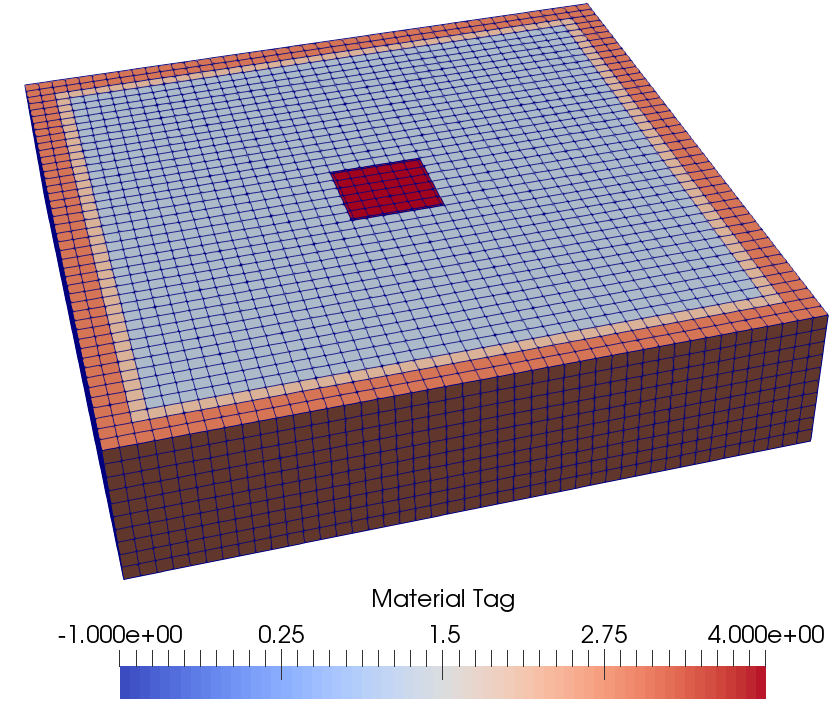
\includegraphics[width = 4cm]{./Figure-files/nonlinear_analysis_steps/soil-foundation/soil_foundation.png}
  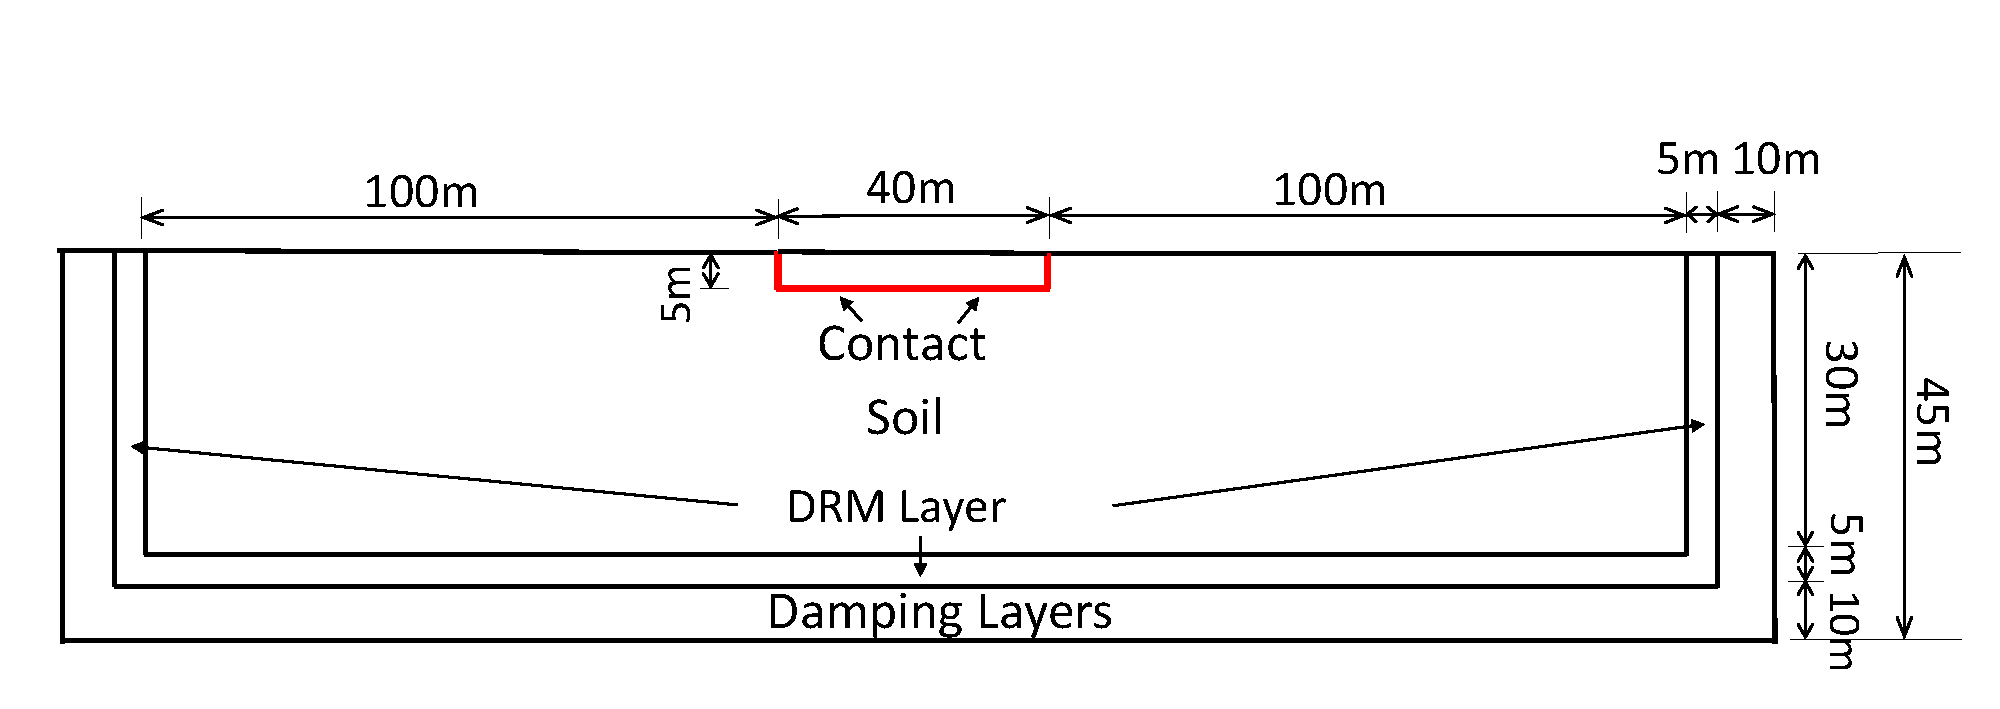
\includegraphics[width = 12cm]{./Figure-files/nonlinear_analysis_steps/soil-foundation/soil_foundation.pdf}
  \caption{Simulation Model}
  \label{fig_foundation_only}
\end{figure}


The illustration results of the simulation is shown in Fig.~\ref{fig_decon_3D_motion_3D_model_results_structure}.
As shown in the results, outside the DRM layer, there is no outgoing waves. 

\begin{figure}[H]
  \centering
  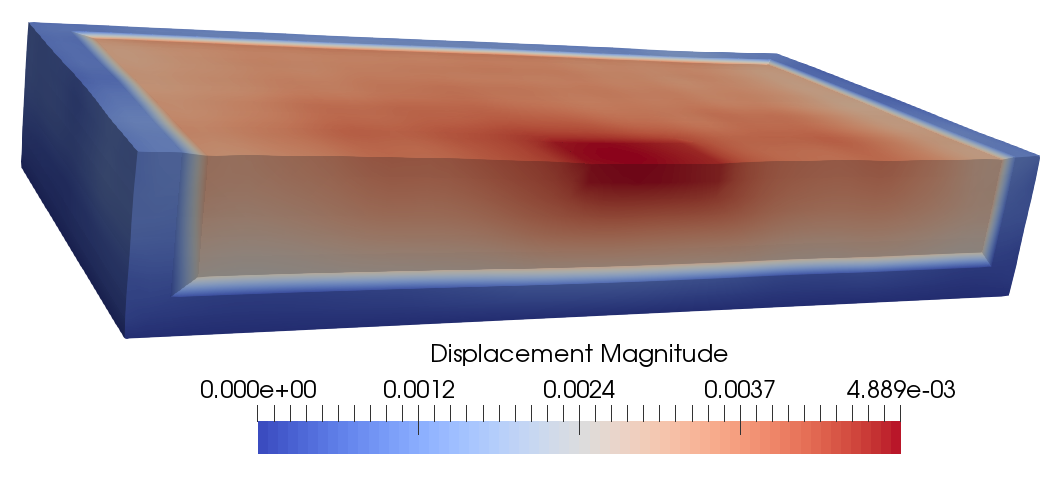
\includegraphics[width = 10cm]{./Figure-files/nonlinear_analysis_steps/soil-foundation/foundation_results.png}
  \caption{Soil Foundation Interaction Results}
  \label{fig_soil_foundation_motion_3D_model_results_structure}
\end{figure}



The node tags of critical points for postprocessing are shown in Fig.\ref{fig_points_soil_foundation}.

\begin{figure}[H]
  \centering
  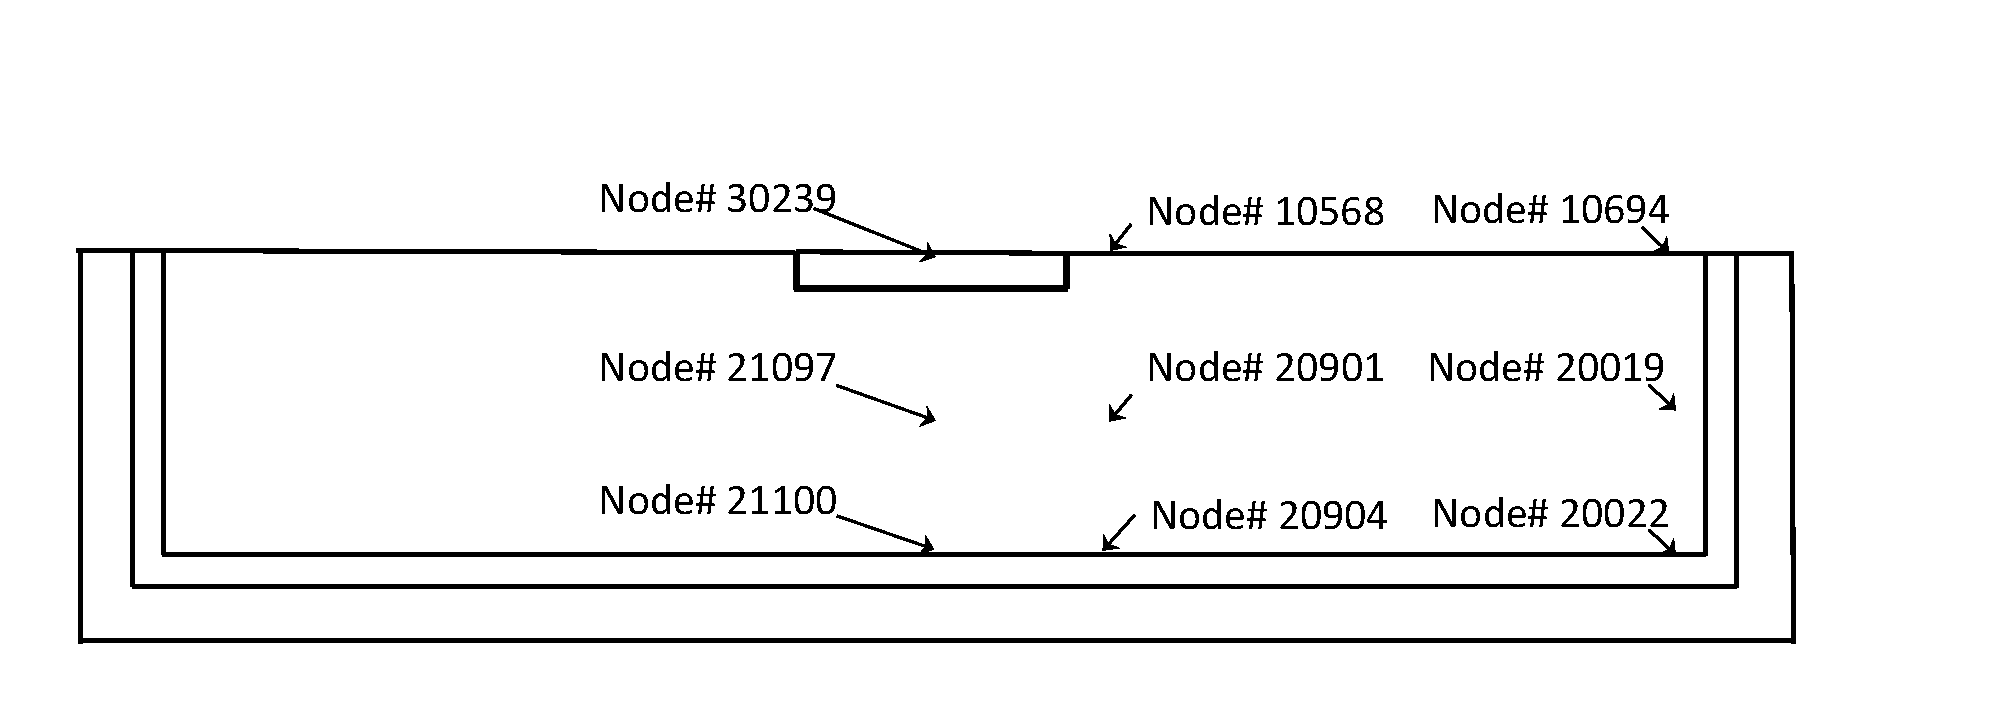
\includegraphics[width = 12cm]{./Figure-files/nonlinear_analysis_steps/soil-foundation/soil_foundation_node_location.pdf}
  \caption{Critical Points of Simulation Model}
  \label{fig_points_soil_foundation}
\end{figure}









% ******************************************************************
% ******************************************************************
% ******************************************************************
\clearpage
\newpage
\section{Soil-Structure Interaction 3D}
\label{ssi_3D}


\paragraph{Elastic Material}
% The Real-ESSI input files for elastic example are available 
% \href{https://github.com/yuan-energy/Real-ESSI-Short-Course-Examples/tree/master/short-course-examples/nonlinear_analysis_steps/soil-structure/elastic}{HERE}. 
The compressed package of input files is  
\href{https://github.com/yuan-energy/Real-ESSI-Short-Course-Examples/tree/master/short-course-examples/nonlinear_analysis_steps/soil-structure/elastic/elastic.tgz?raw=true}{HERE}. 

The Modeling parameters are listed.
\begin{itemize}
  \item Elastic Material Properties 
  \begin{itemize}
    \item Mass density, $\rho$, \enspace \enspace 2000 $kg/m^3$
    \item Young's modulus, $E$, \enspace \enspace 1.1 GPa
    \item Poisson's ratio, $\nu$, \enspace \enspace 0.1
  \end{itemize}
\end{itemize}


SIMULATION TIME: With 8 cores on AWS EC2 c4.2xlarge instance, the running time for this example is 10 minutes.

\paragraph{von-Mises Armstrong-Frederick Material}
% The Real-ESSI input files for this example are available 
% \href{https://github.com/yuan-energy/Real-ESSI-Short-Course-Examples/tree/master/short-course-examples/nonlinear_analysis_steps/soil-structure/vonMisesArmstrongFrederick}{HERE}. 
The compressed package of input files is  
\href{https://github.com/yuan-energy/Real-ESSI-Short-Course-Examples/tree/master/short-course-examples/nonlinear_analysis_steps/soil-structure/vonMisesArmstrongFrederick/vonMisesArmstrongFrederick.tgz?raw=true}{HERE}. 


The Modeling parameters are listed.
\begin{itemize}
  \item von-Mises nonlinear hardening material model 
  \begin{itemize}
    \item Mass density, $\rho$, \enspace \enspace 2000 $kg/m^3$
    \item Young's modulus, $E$, \enspace \enspace 1.1 GPa
    \item Poisson's ratio, $\nu$, \enspace \enspace 0.1
    \item von Mises radius, $k$, \enspace \enspace 60 kPa
    \item nonlinear kinematic hardening rate, $H_a$, \enspace \enspace  30 MPa
    \item nonlinear kinematic hardening rate, $C_r$, \enspace \enspace  25
    \item isotropic hardening rate, $K_{iso}$, \enspace \enspace 0 Pa
  \end{itemize}
\end{itemize}


SIMULATION TIME: With 8 cores on AWS EC2 c4.2xlarge instance, the running time for this example is 46 minutes.

\paragraph{von-Mises G/Gmax Material}
% The Real-ESSI input files for this example are available 
% \href{https://github.com/yuan-energy/Real-ESSI-Short-Course-Examples/tree/master/short-course-examples/nonlinear_analysis_steps/soil-structure/vonMisesGoverGmax}{HERE}. 
The compressed package of input files is  
\href{https://github.com/yuan-energy/Real-ESSI-Short-Course-Examples/tree/master/short-course-examples/nonlinear_analysis_steps/soil-structure/vonMisesGoverGmax/vonMisesGoverGmax.tgz?raw=true}{HERE}. 

The Modeling parameters are listed.
\begin{itemize}
  \item von-Mises G/Gmax material model 
  \begin{itemize}
    \item Mass density, $\rho$, \enspace \enspace 2000 $kg/m^3$
    \item Young's modulus, $E$, \enspace \enspace 1.1 GPa
    \item Poisson's ratio, $\nu$, \enspace \enspace 0.1
    \item Total number of shear modulus \enspace \enspace  9
    \item G over Gmax, \enspace \enspace  1,0.995,0.966,0.873,0.787,0.467,0.320,0.109,0.063
    \item Shear strain gamma, \enspace \enspace  0,1E-6,1E-5,5E-5,1E-4, 0.0005, 0.001, 0.005, 0.01
  \end{itemize}
\end{itemize}

SIMULATION TIME: With 8 cores on AWS EC2 c4.2xlarge instance, the running time for this example is 755 minutes.

\paragraph{Drucker-Prager G/Gmax Material}
% The Real-ESSI input files for this example are available 
% \href{https://github.com/yuan-energy/Real-ESSI-Short-Course-Examples/tree/master/short-course-examples/nonlinear_analysis_steps/soil-structure/DruckerPragerGoverGmax}{HERE}. 
The compressed package of input files is  
\href{https://github.com/yuan-energy/Real-ESSI-Short-Course-Examples/tree/master/short-course-examples/nonlinear_analysis_steps/soil-structure/DruckerPragerGoverGmax/DruckerPragerGoverGmax.tgz?raw=true}{HERE}. 

SIMULATION TIME: With 8 cores on AWS EC2 c4.2xlarge instance, the running time for this example is 1178 minutes.

The Modeling parameters are listed.
\begin{itemize}
  \item Drucker-Prager G/Gmax material model 
  \begin{itemize}
    \item Mass density, $\rho$, \enspace \enspace 2000 $kg/m^3$
    \item Young's modulus, $E$, \enspace \enspace 1.1 GPa
    \item Poisson's ratio, $\nu$, \enspace \enspace 0.1
    \item Initial confining stress, $p_0$, \enspace \enspace 100 kPa
    \item Reference pressure, $p_{refer} $, \enspace \enspace 100 kPa
    \item Pressure exponential, $ n  $, \enspace \enspace 0.5
    \item Cohesion, $ n  $, \enspace \enspace 1 kPa
    \item Total number of Shear Modulus \enspace \enspace 9
    \item G over Gmax, \enspace \enspace  1,0.995,0.966,0.873,0.787,0.467,0.320,0.109,0.063
    \item Shear strain gamma, \enspace \enspace  0,1E-6,1E-5,5E-5,1E-4, 0.0005, 0.001, 0.005, 0.01
  \end{itemize}
\end{itemize}

% SIMULATION TIME: With 8 cores, the running time for this example is 

\paragraph{Contact Elements}
% The Real-ESSI input files for this example are available 
% \href{https://github.com/yuan-energy/Real-ESSI-Short-Course-Examples/tree/master/short-course-examples/nonlinear_analysis_steps/soil-structure/contact}{HERE}. 
The compressed package of input files is  
\href{https://github.com/yuan-energy/Real-ESSI-Short-Course-Examples/tree/master/short-course-examples/nonlinear_analysis_steps/soil-structure/contact/contact.tgz?raw=true}{HERE}. 

SIMULATION TIME: With 8 cores on AWS EC2 c4.2xlarge instance, the running time for this example is 15 minutes.

\paragraph{Both Elastoplastic Material and Contact Elements}
% The Real-ESSI input files for both elastoplastic material and contact element example are available 
% \href{https://github.com/yuan-energy/Real-ESSI-Short-Course-Examples/tree/master/short-course-examples/nonlinear_analysis_steps/soil-structure/both_plastic_contact}{HERE}. 
The compressed package of input files is  
\href{https://github.com/yuan-energy/Real-ESSI-Short-Course-Examples/tree/master/short-course-examples/nonlinear_analysis_steps/soil-structure/both_plastic_contact/both_plastic_contact.tgz?raw=true}{HERE}. 





The thickness of the shell structure is 2 meters.

\begin{figure}[H]
  \centering
  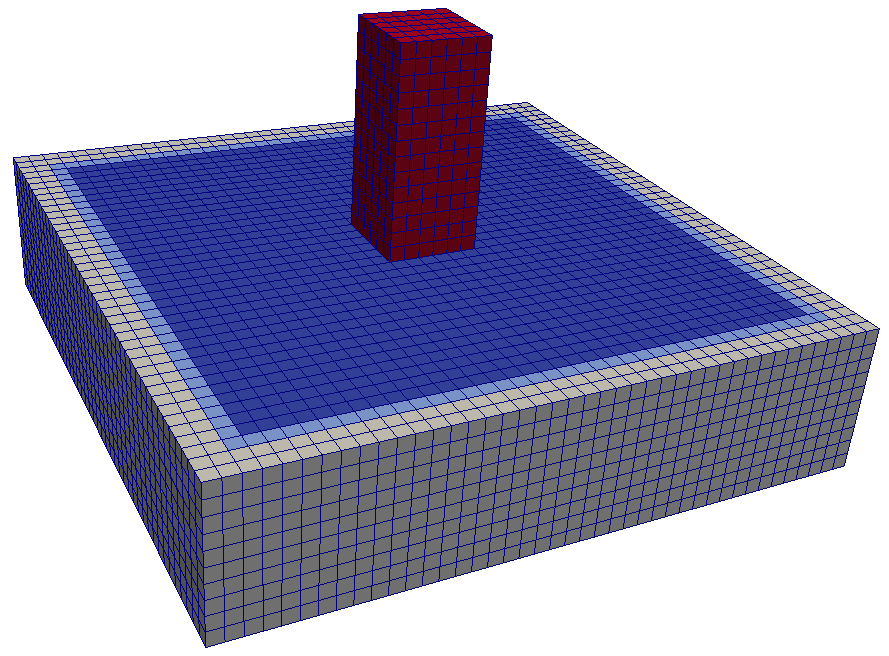
\includegraphics[width = 7cm]{./Figure-files/nonlinear_analysis_steps/soil-structure/overview.png}
  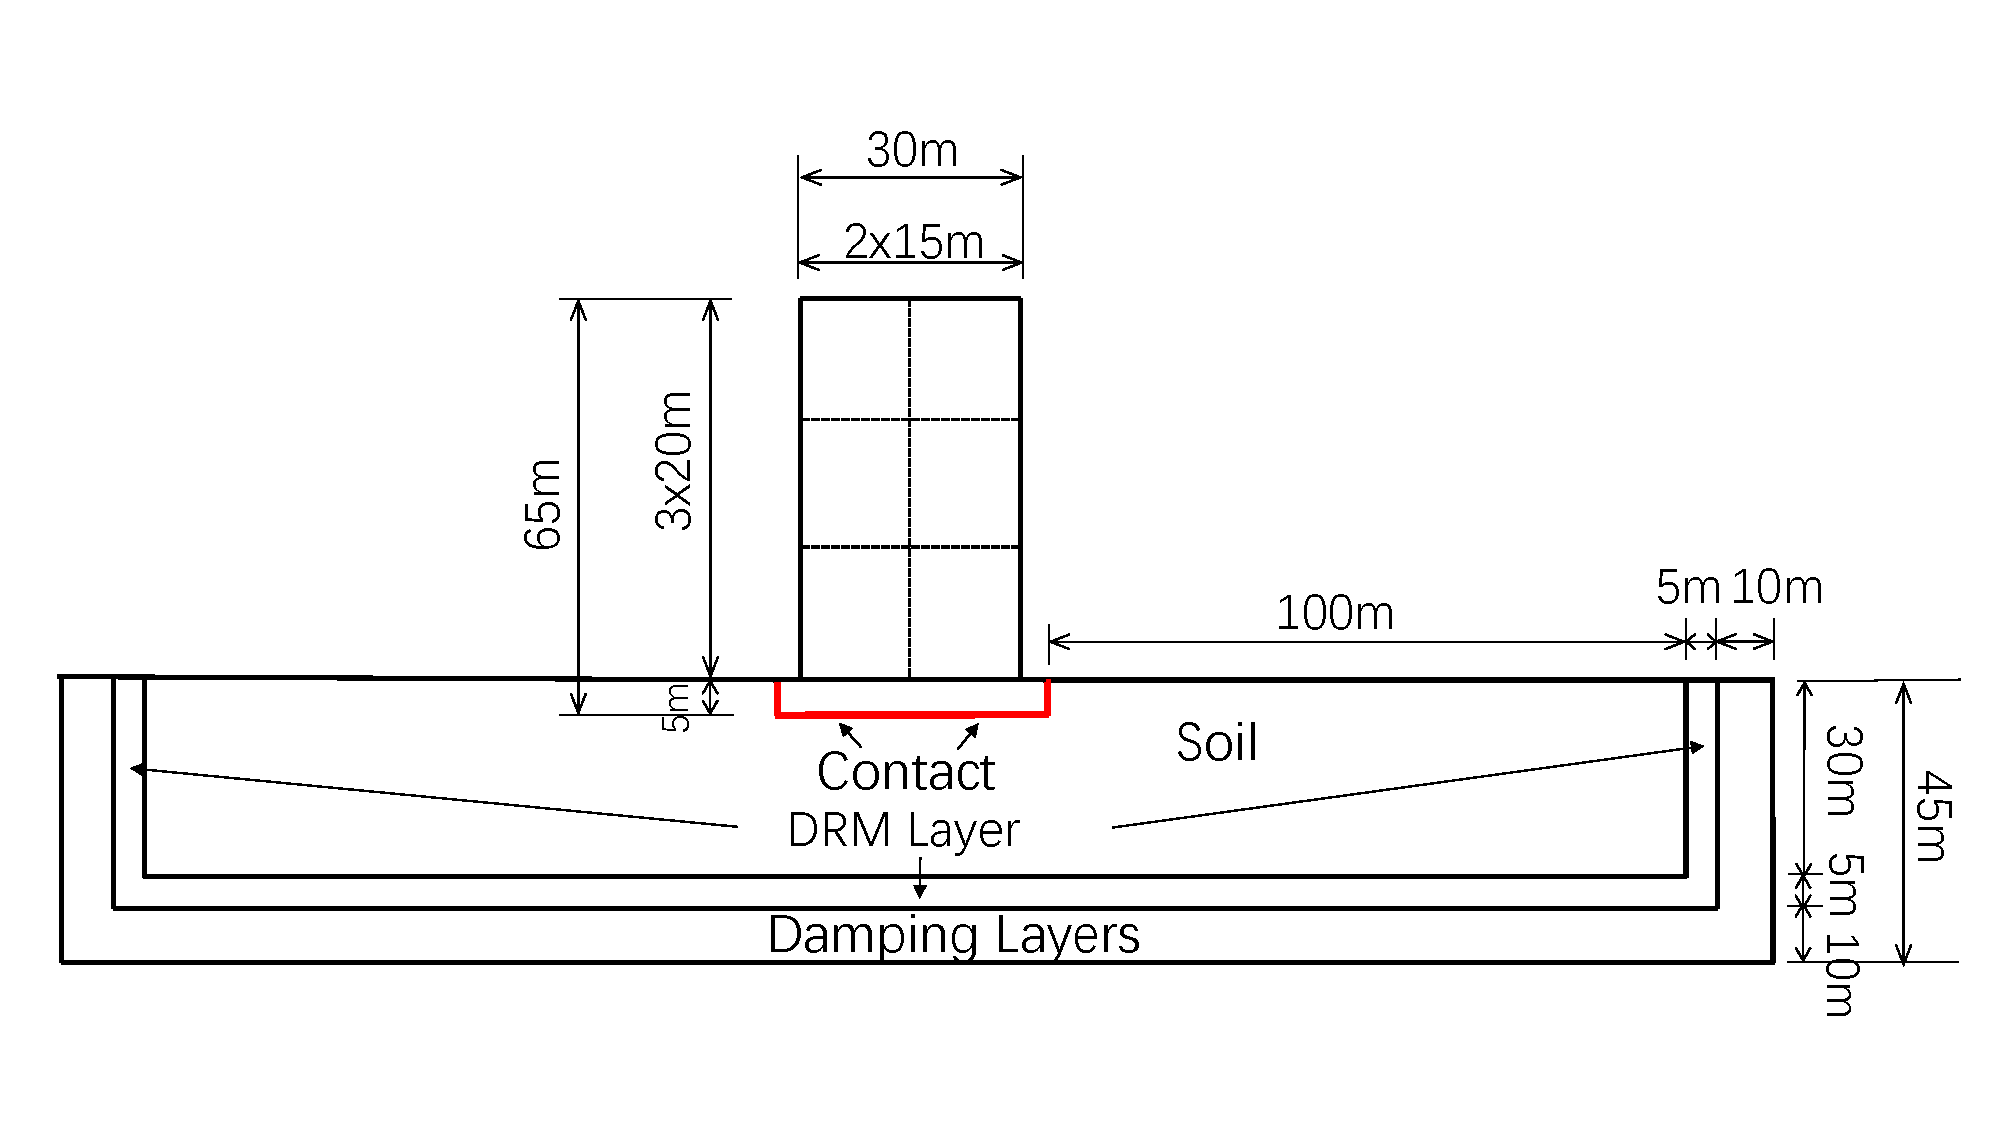
\includegraphics[width = 14cm]{./Figure-files/nonlinear_analysis_steps/soil-structure/geometry.pdf}
  \caption{Simulation Model}
  \label{fig_decon_1D_motion_3D_model}
\end{figure}


The illustration results of the simulation is shown in Fig.~\ref{fig_decon_3D_motion_3D_model_results_structure}.
As shown in the results, outside the DRM layer, there is no outgoing waves. 

\begin{figure}[H]
  \centering
  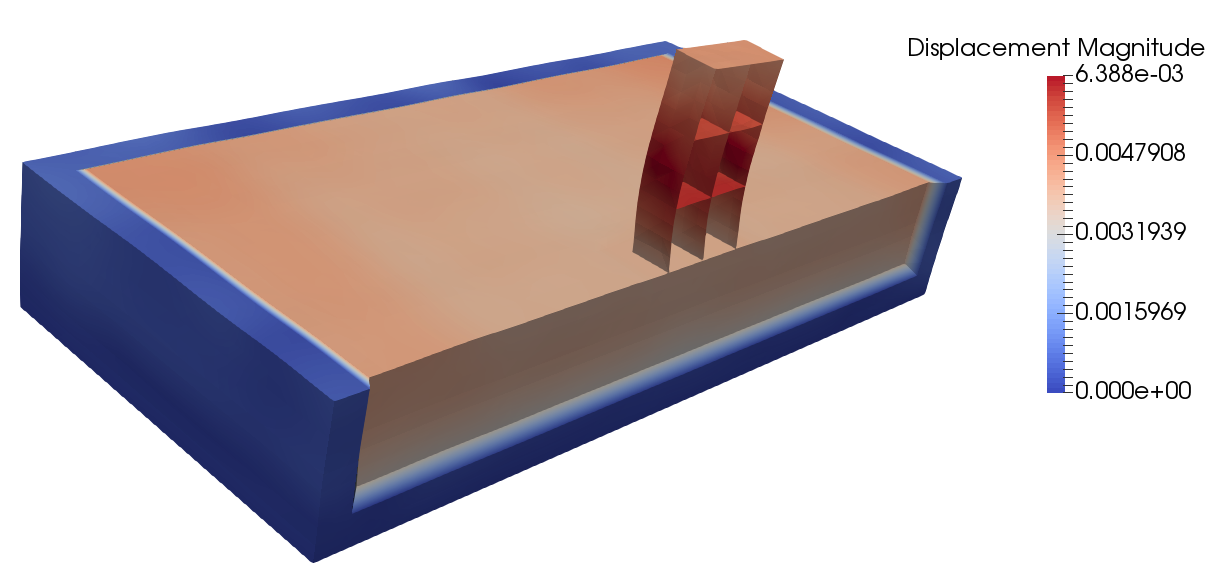
\includegraphics[width = 12cm]{./Figure-files/nonlinear_analysis_steps/soil-structure/DRM3D_motion3D_structure.png}
  \caption{Simulation Model}
  \label{fig_decon_3D_motion_3D_model_results_structure}
\end{figure}

The node tags of critical points for postprocessing are shown in Fig.\ref{fig_points_3D_motion_3D_model_results_structure}.

\begin{figure}[H]
  \centering
  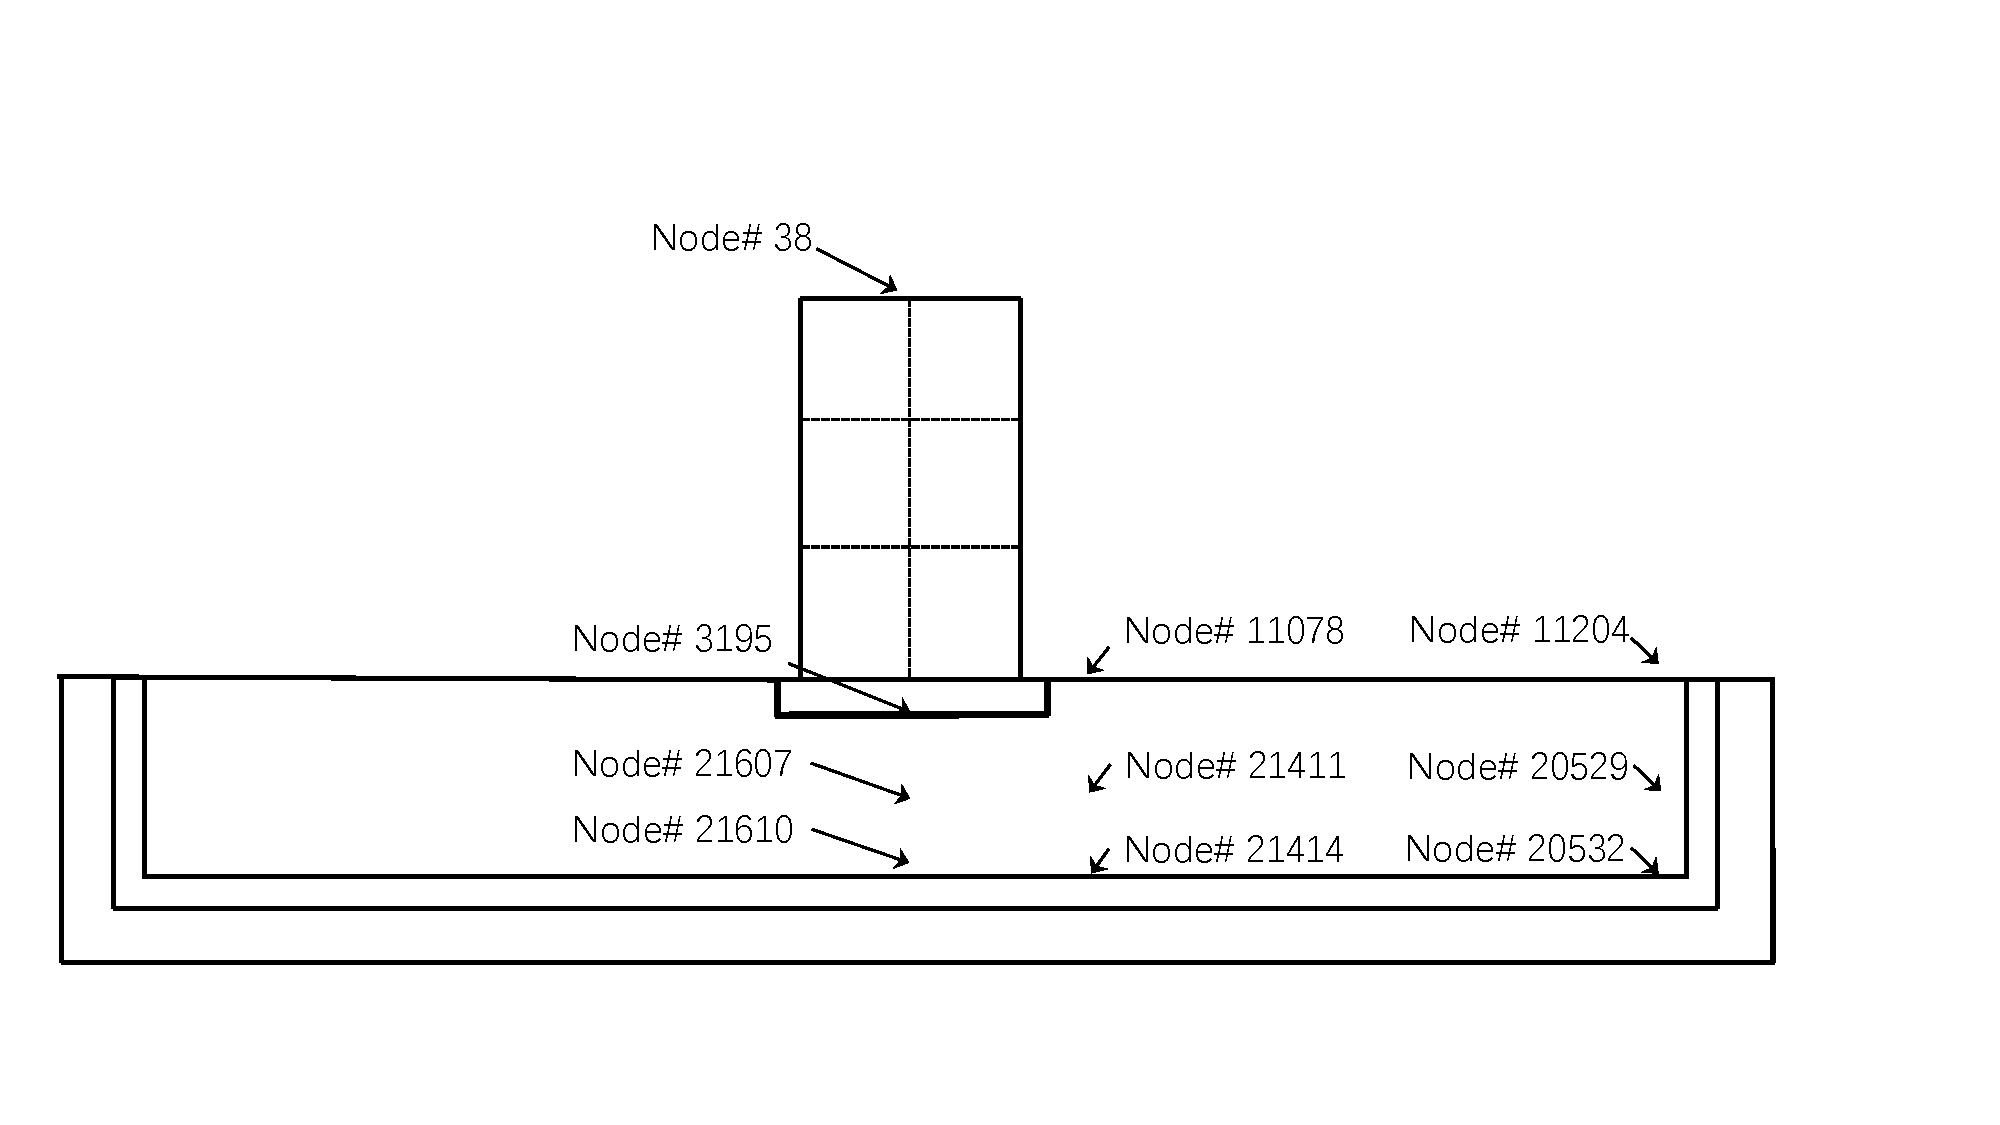
\includegraphics[width = 12cm]{./Figure-files/nonlinear_analysis_steps/soil-structure/soil-structure_node_location.pdf}
  \caption{Critical Points of Simulation Model}
  \label{fig_points_3D_motion_3D_model_results_structure}
\end{figure}

SIMULATION TIME: With 8 cores on AWS EC2 c4.2xlarge instance, the running time for this example is 47 minutes.

\paragraph{Simulation with 1D motion }
The time series of simulation results is shown in Fig.~\ref{fig_decon_3D_motion_1D_model_results_top_bottom_time_series_ssi3d_1D_motion}.
\begin{figure}[H]
  \centering
  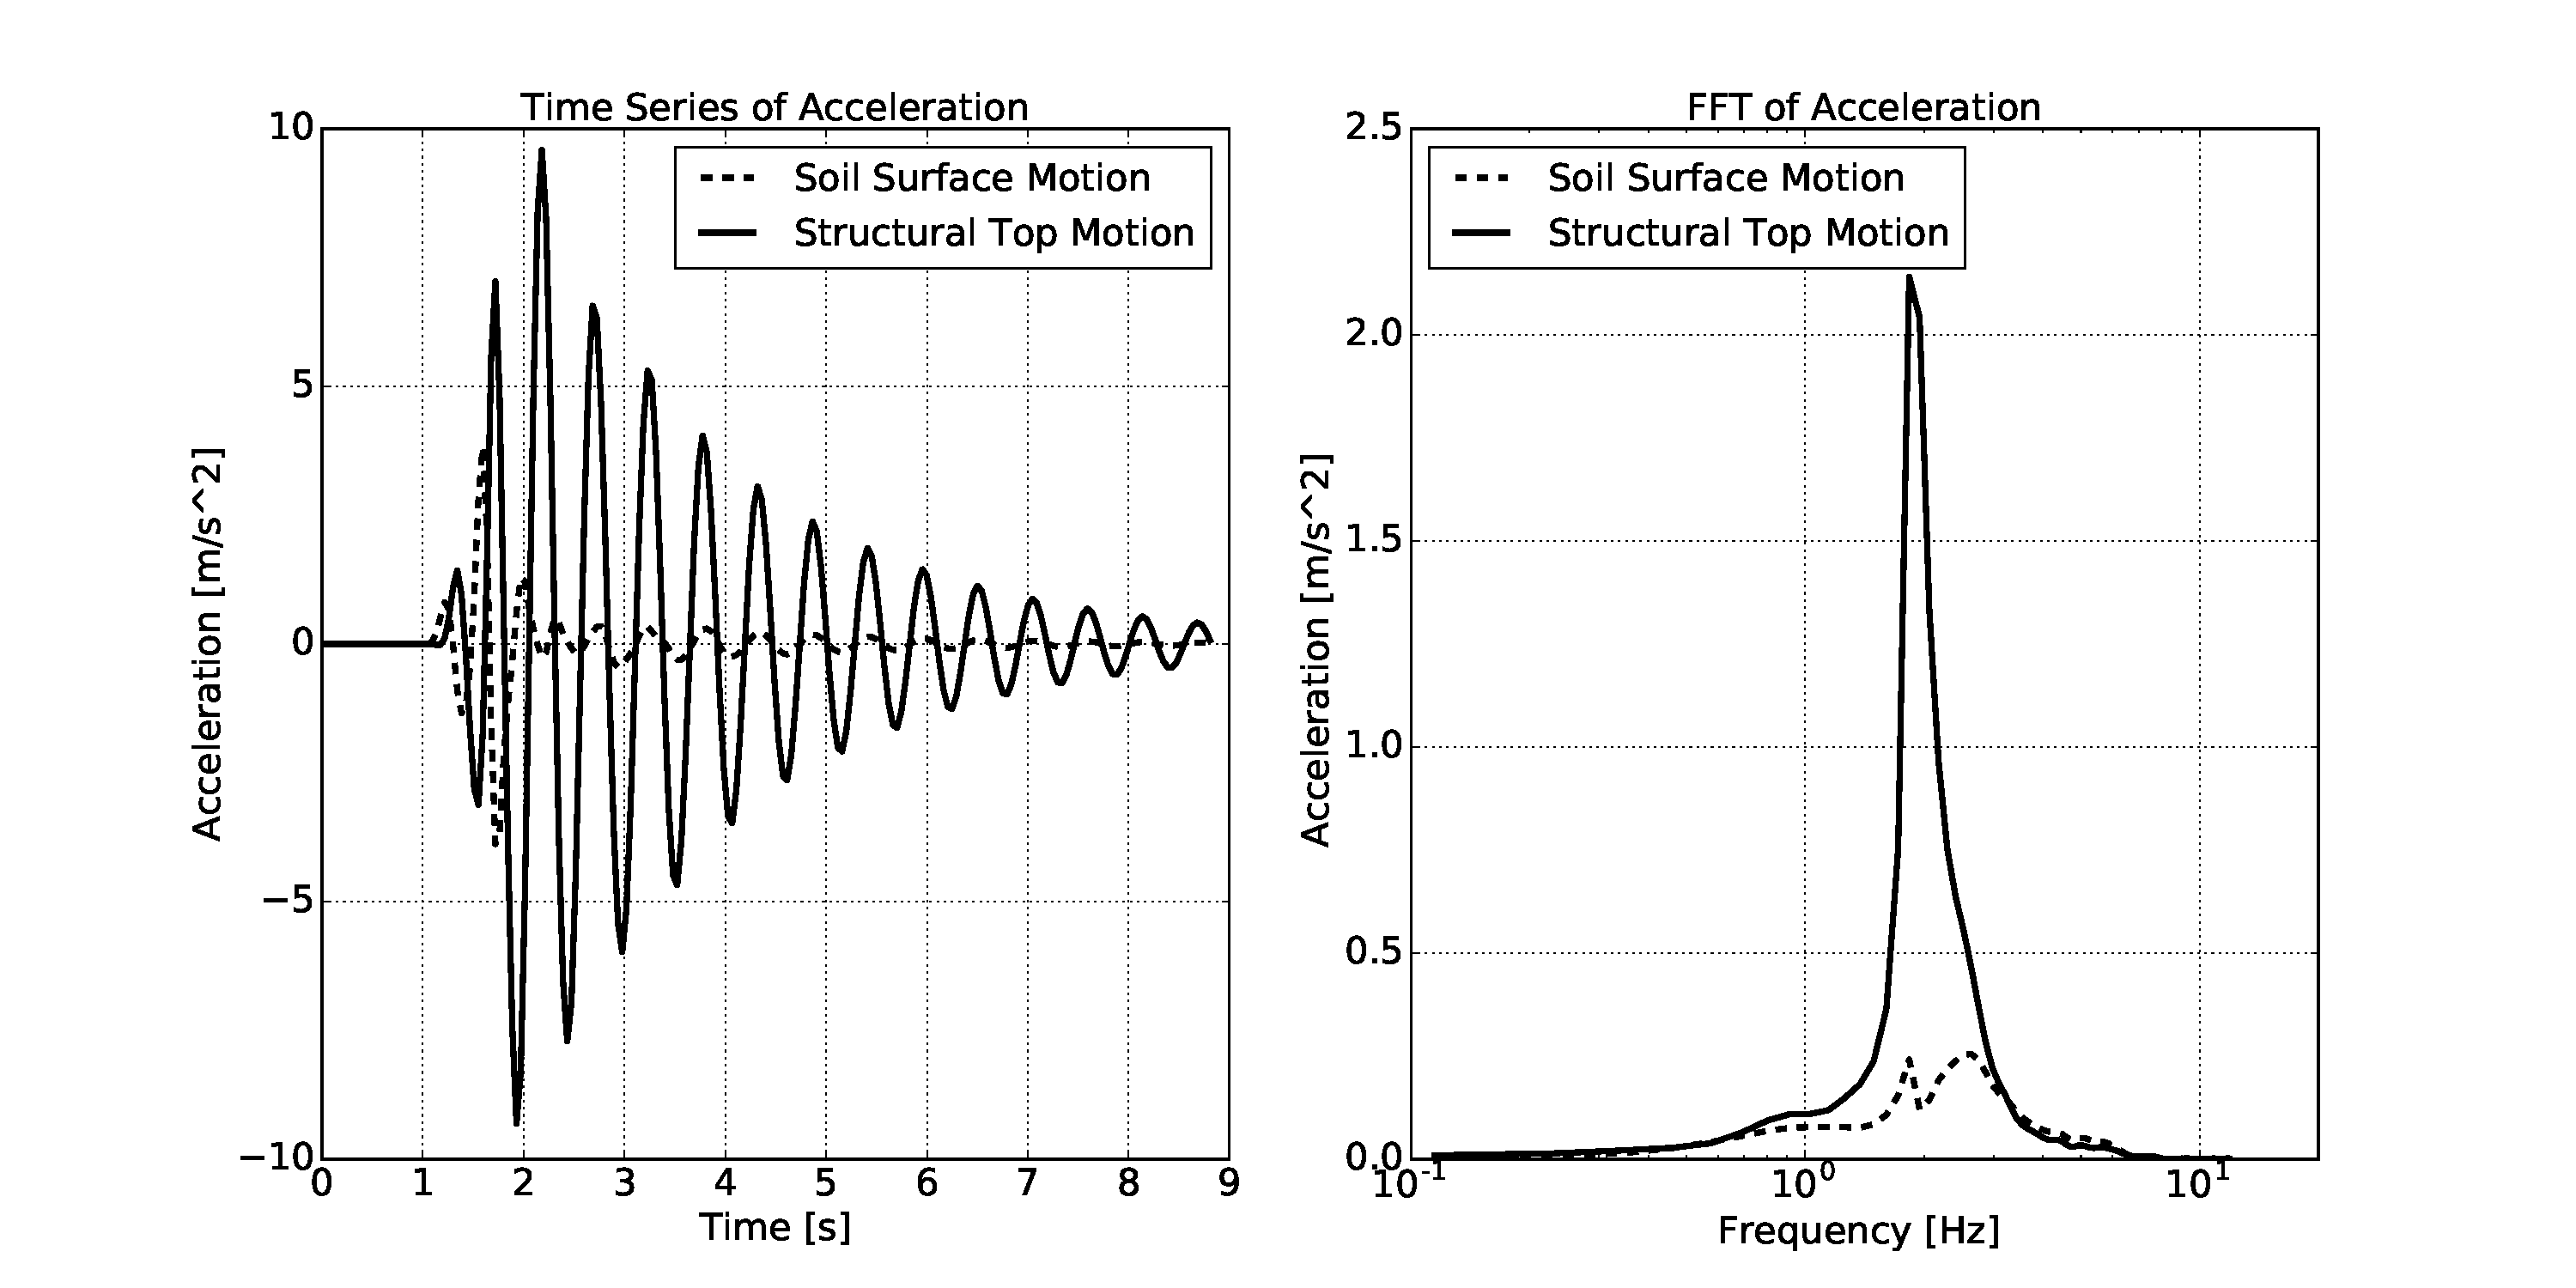
\includegraphics[width = 15cm]{./Figure-files/nonlinear_analysis_steps/soil-structure-1D-ans/shell_structure_motion_node_38_x_acce_compare.pdf}
  \caption{Simulation Results: time series under 1D motion}
  \label{fig_decon_3D_motion_1D_model_results_top_bottom_time_series_ssi3d_1D_motion}
\end{figure}

The response spectrum of motion is shown in Fig.~\ref{fig_spectrum_freq_period_time_series_ssi3d_1D_motion}.
\begin{figure}[H]
  \centering
  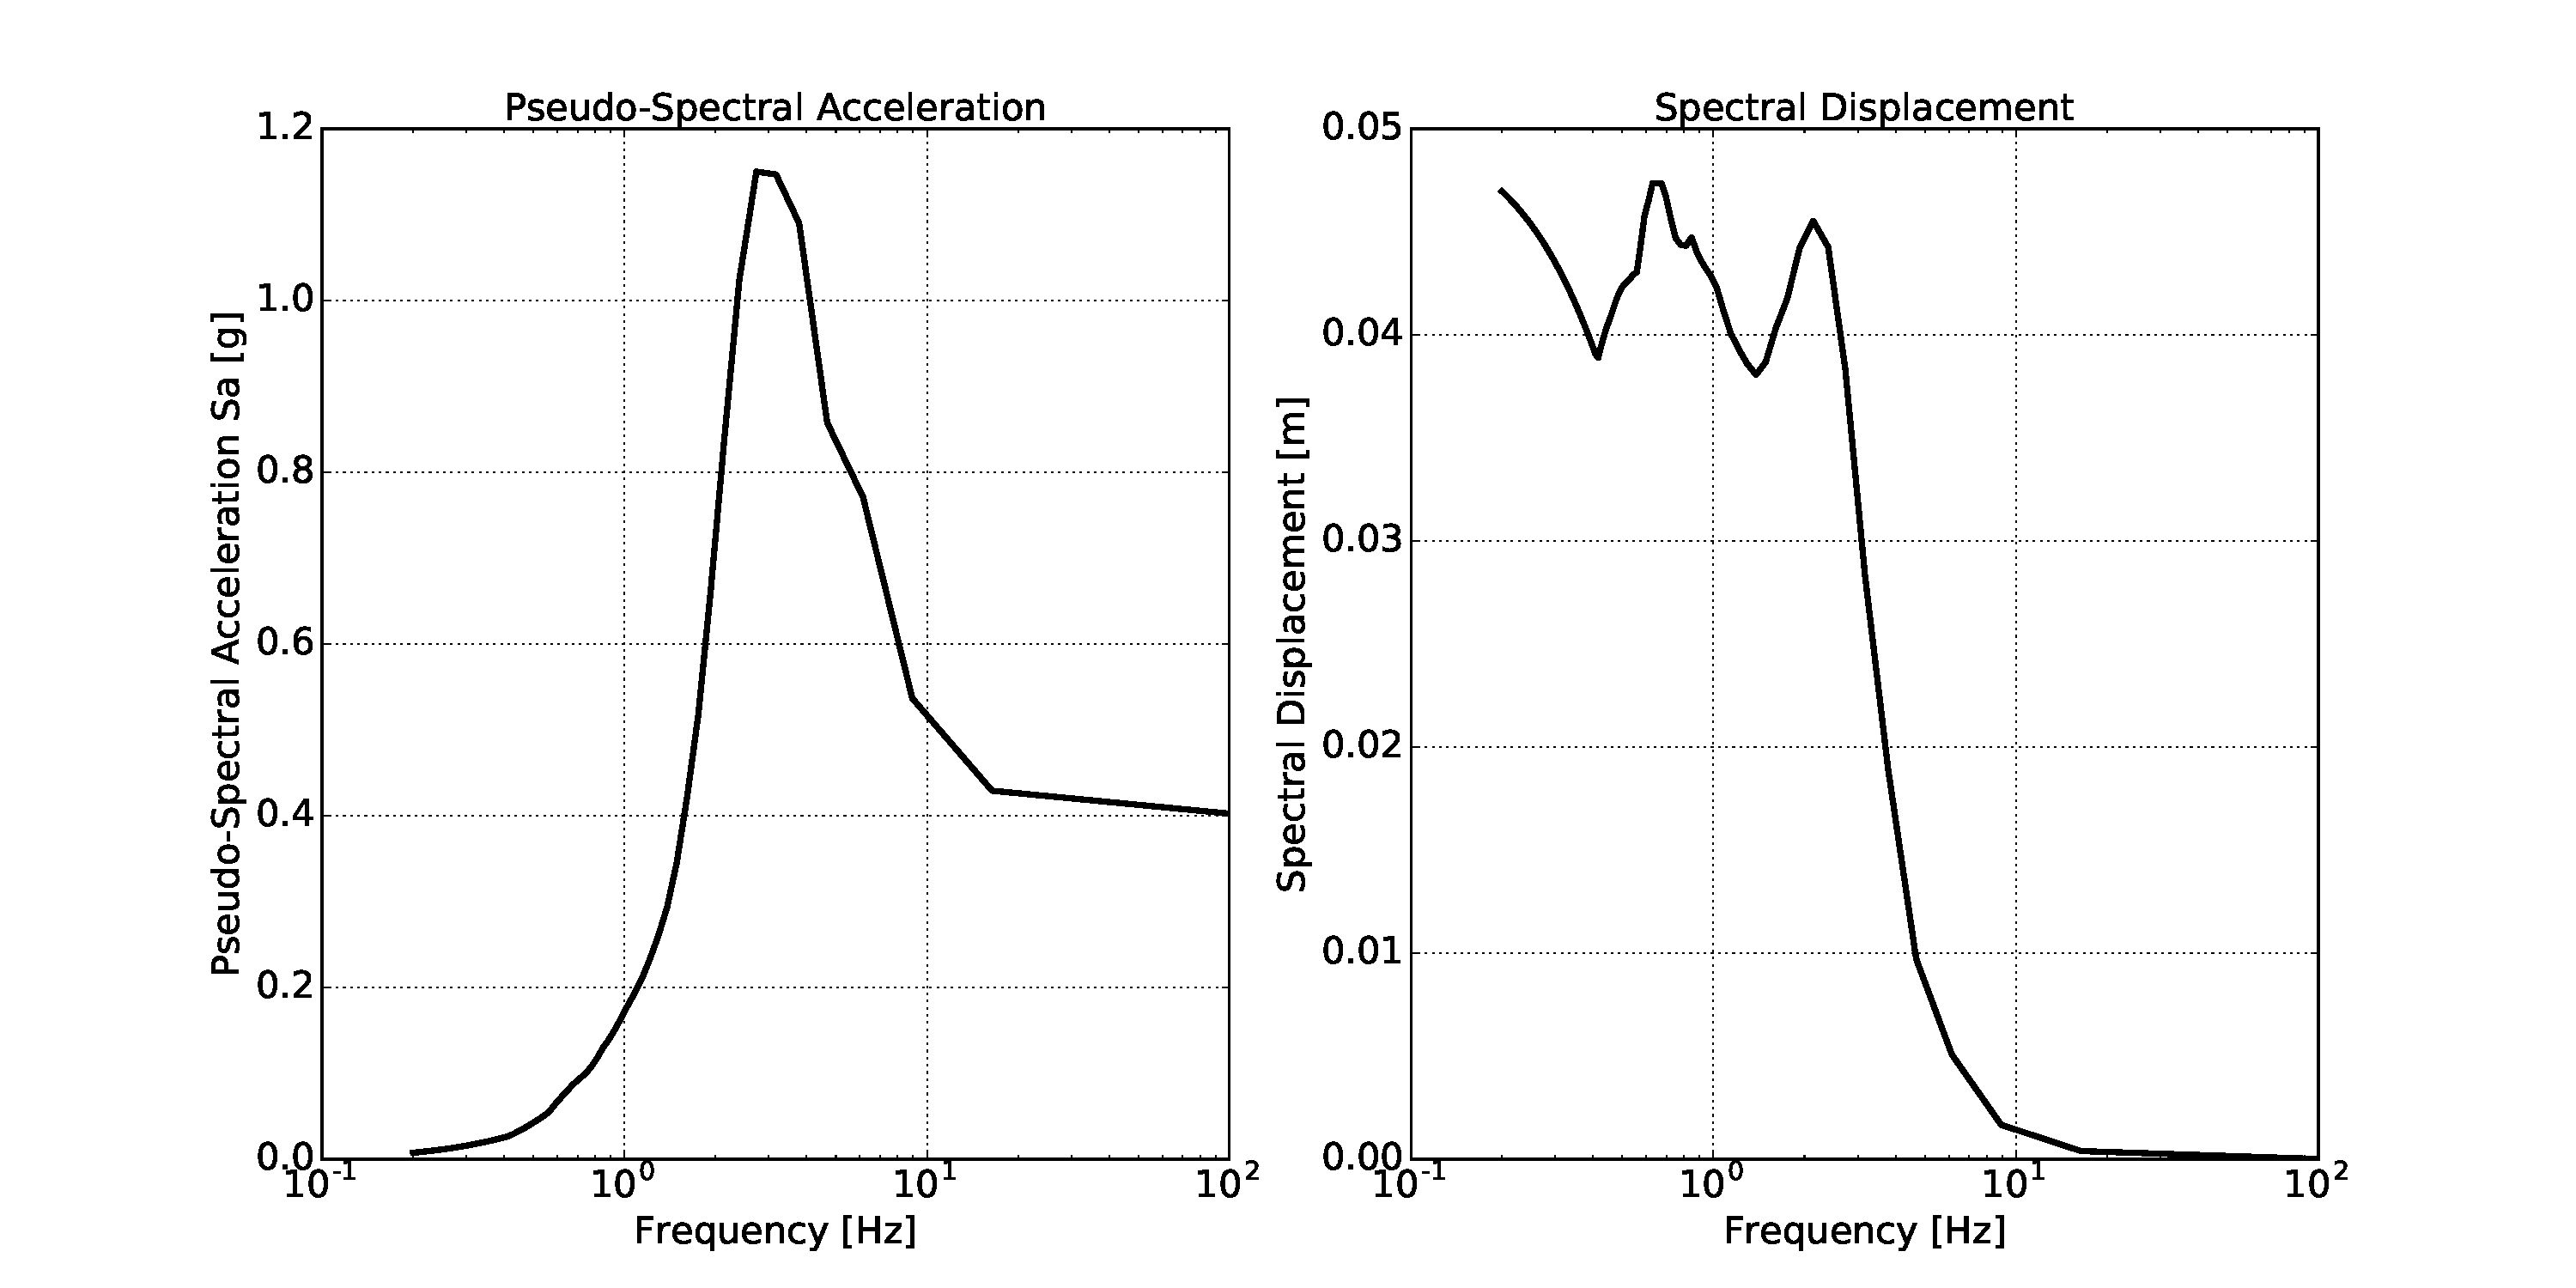
\includegraphics[width = 15cm]{./Figure-files/nonlinear_analysis_steps/soil-structure-1D-ans/shell_structure_motion_node_3195_x_spectrum_freq.pdf}
  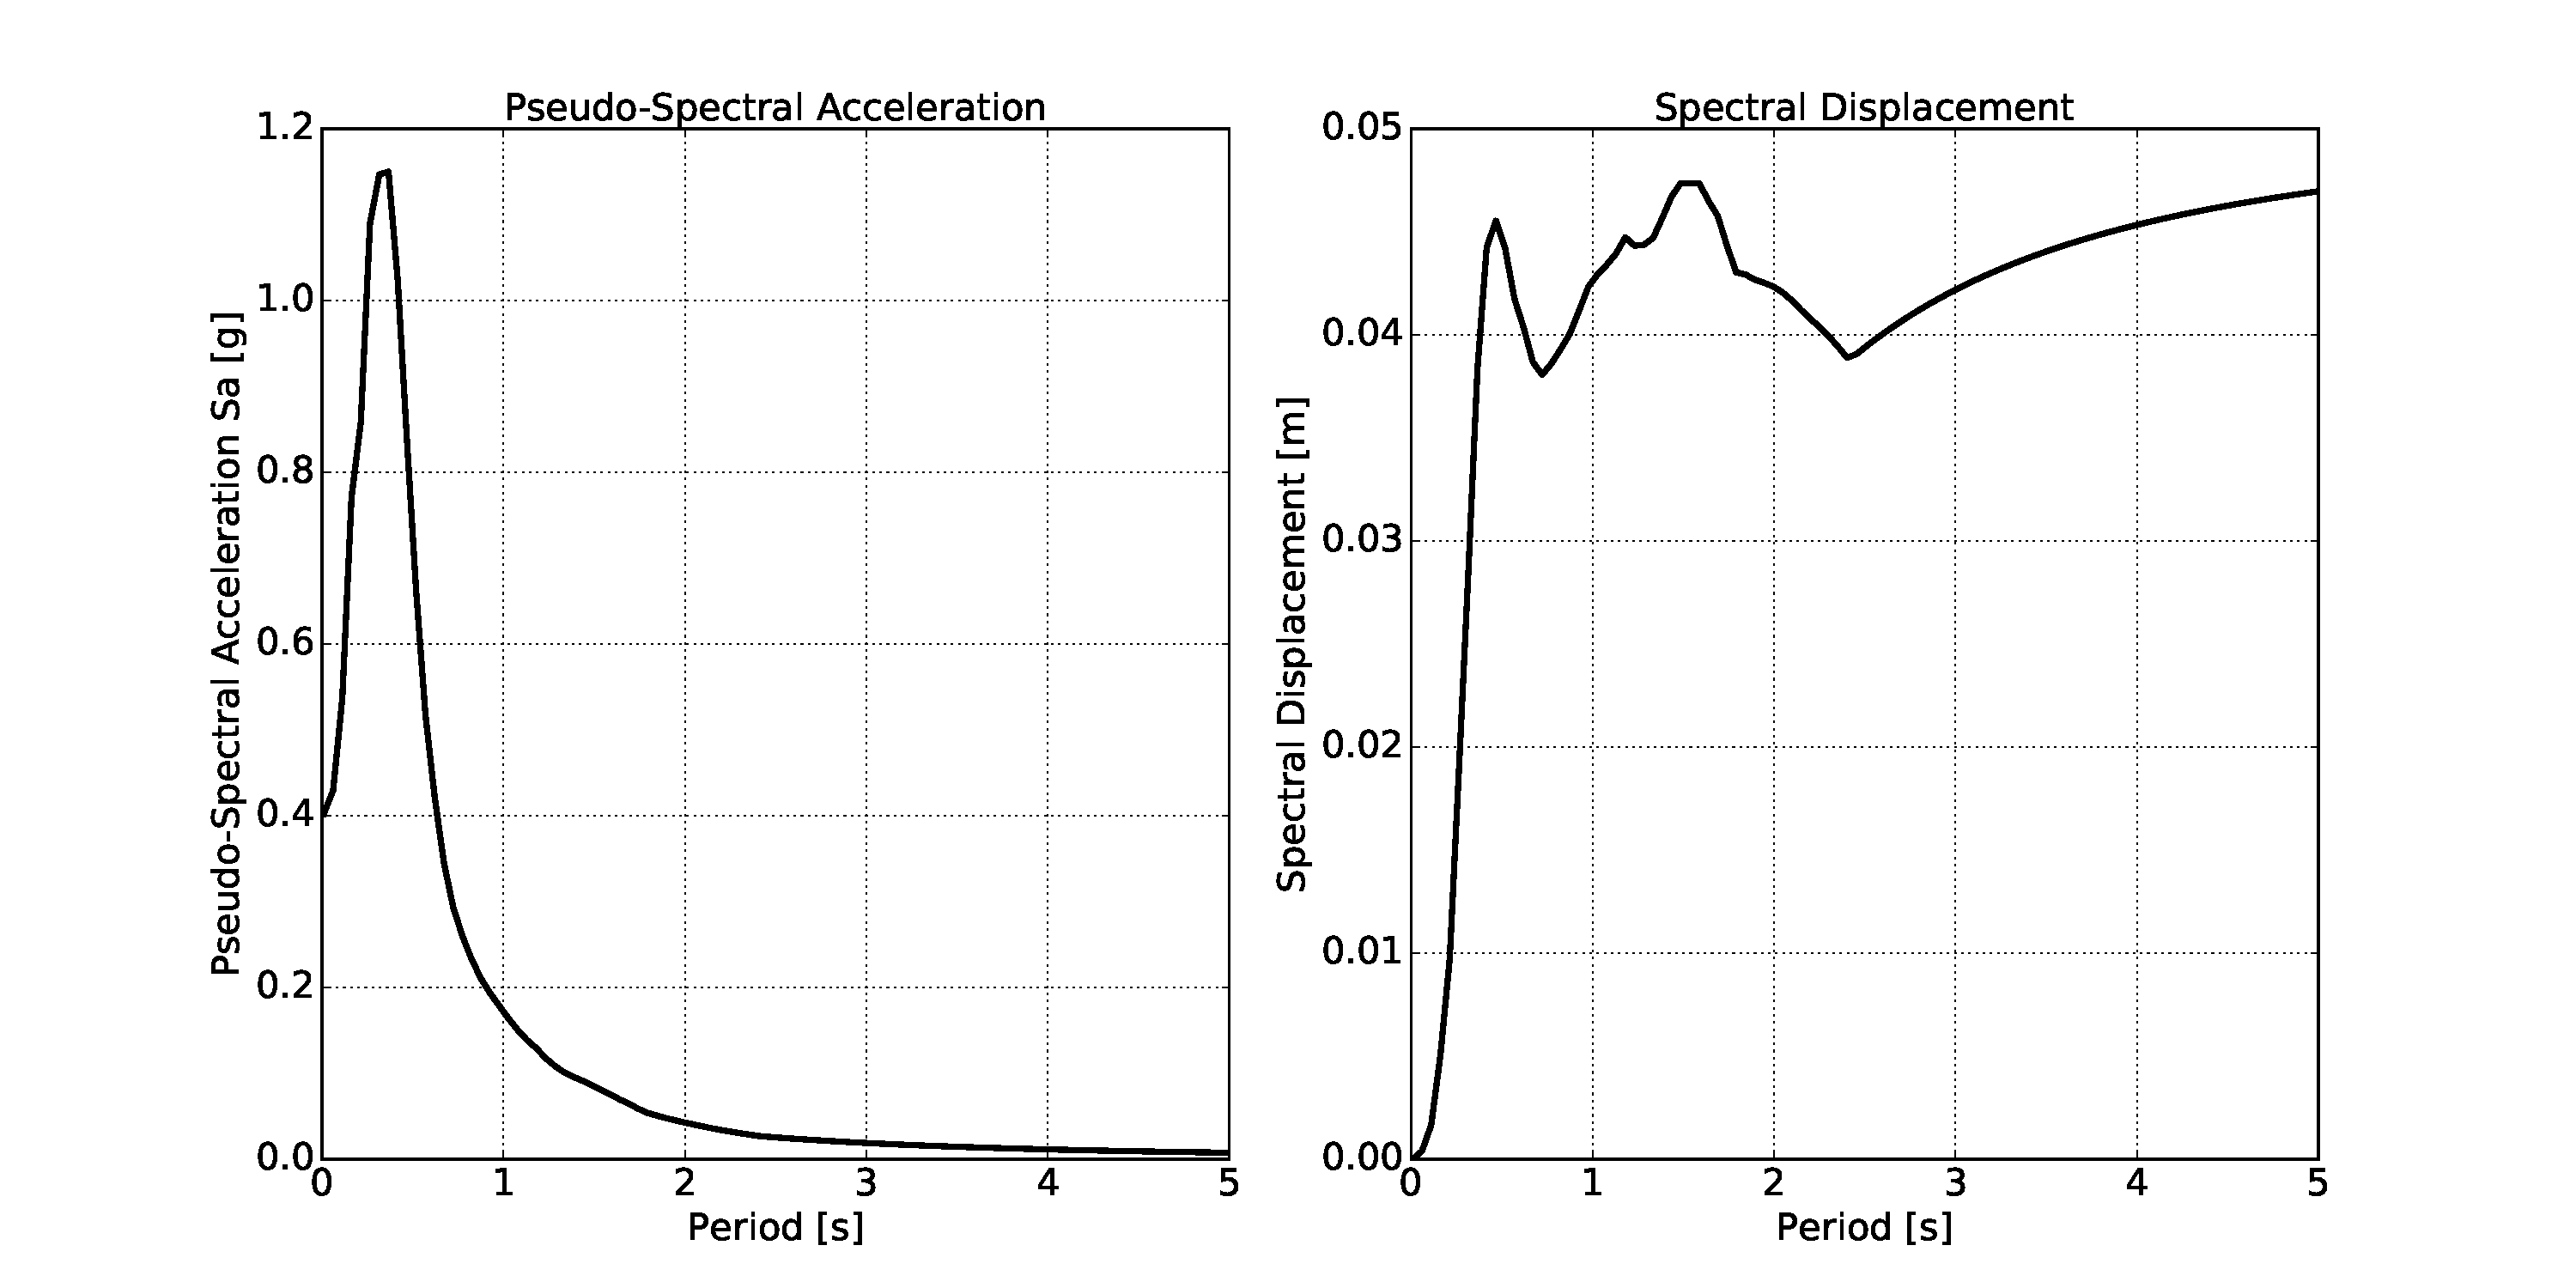
\includegraphics[width = 15cm]{./Figure-files/nonlinear_analysis_steps/soil-structure-1D-ans/shell_structure_motion_node_3195_x_spectrum_period.pdf}
  \caption{Simulation Results: Response Spectrum under 1D motion}
  \label{fig_spectrum_freq_period_time_series_ssi3d_1D_motion}
\end{figure}


\paragraph{Simulation with 3 $\times$ 1D motion }
The time series of simulation results is shown in Fig.~\ref{fig_decon_3D_motion_1D_model_results_top_bottom_time_series_ssi3d_3D_motion}.
\begin{figure}[H]
  \centering
  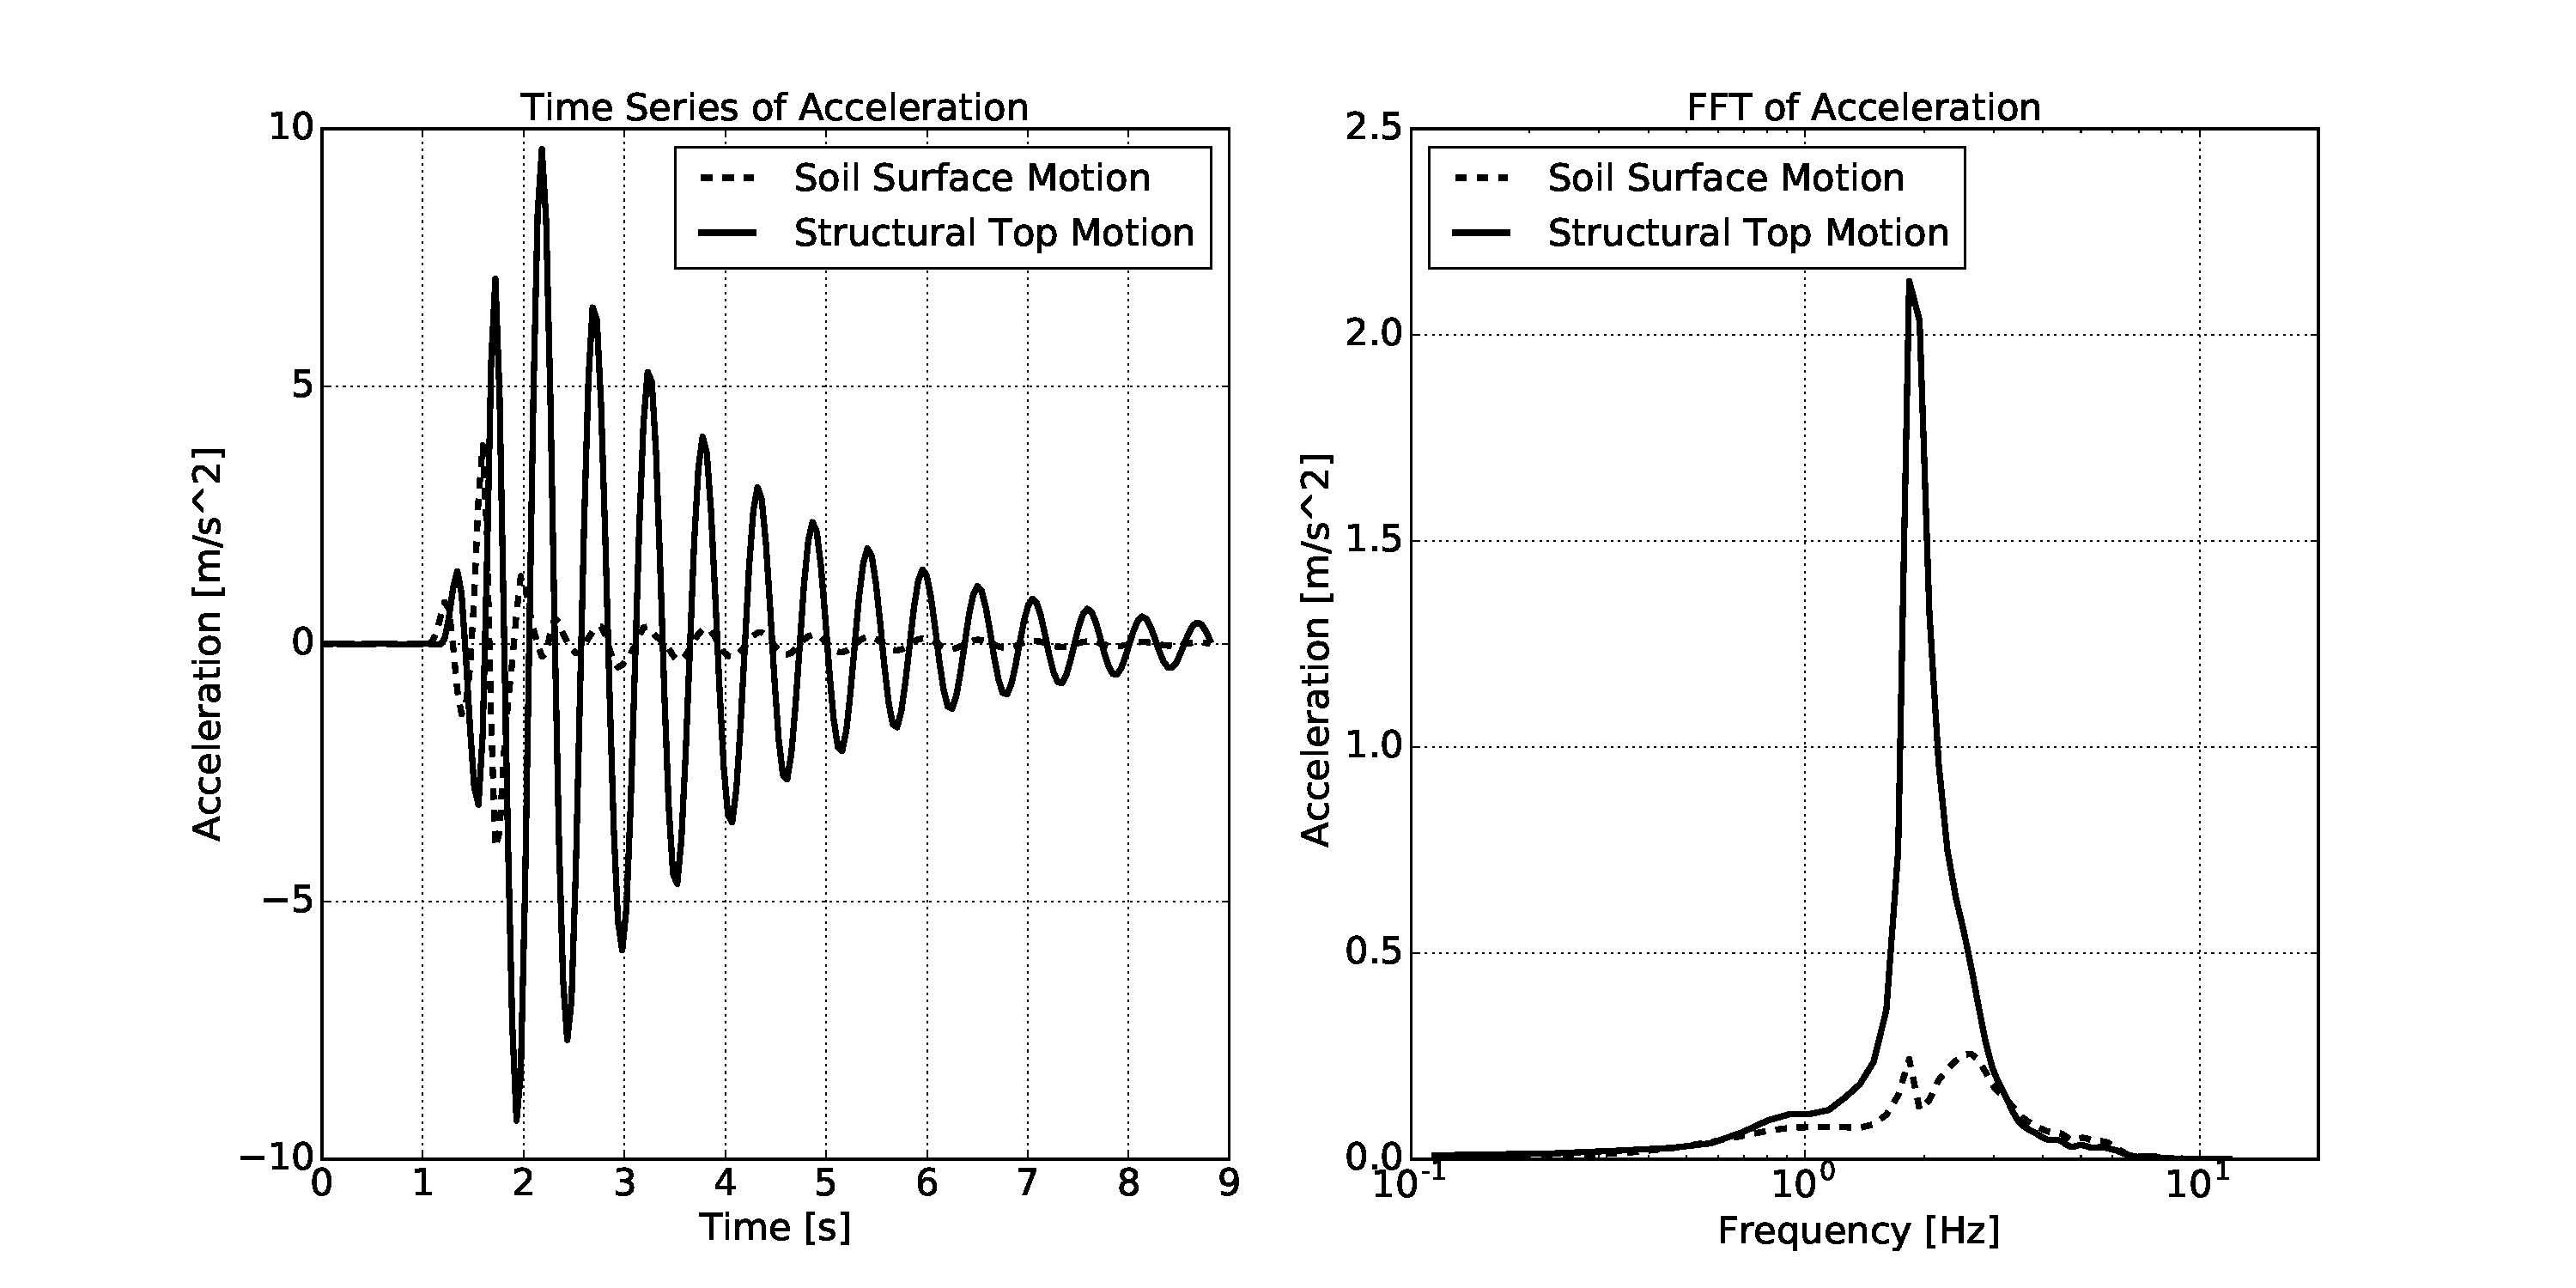
\includegraphics[width = 15cm]{./Figure-files/nonlinear_analysis_steps/soil-structure-3D-ans/shell_structure_motion_node_38_x_acce_compare.pdf}
  \caption{Simulation Results: time series under 3D motion}
  \label{fig_decon_3D_motion_1D_model_results_top_bottom_time_series_ssi3d_3D_motion}
\end{figure}

The response spectrum of motion is shown in Fig.~\ref{fig_spectrum_freq_period_time_series_ssi3d_3D_motion}.
\begin{figure}[H]
  \centering
  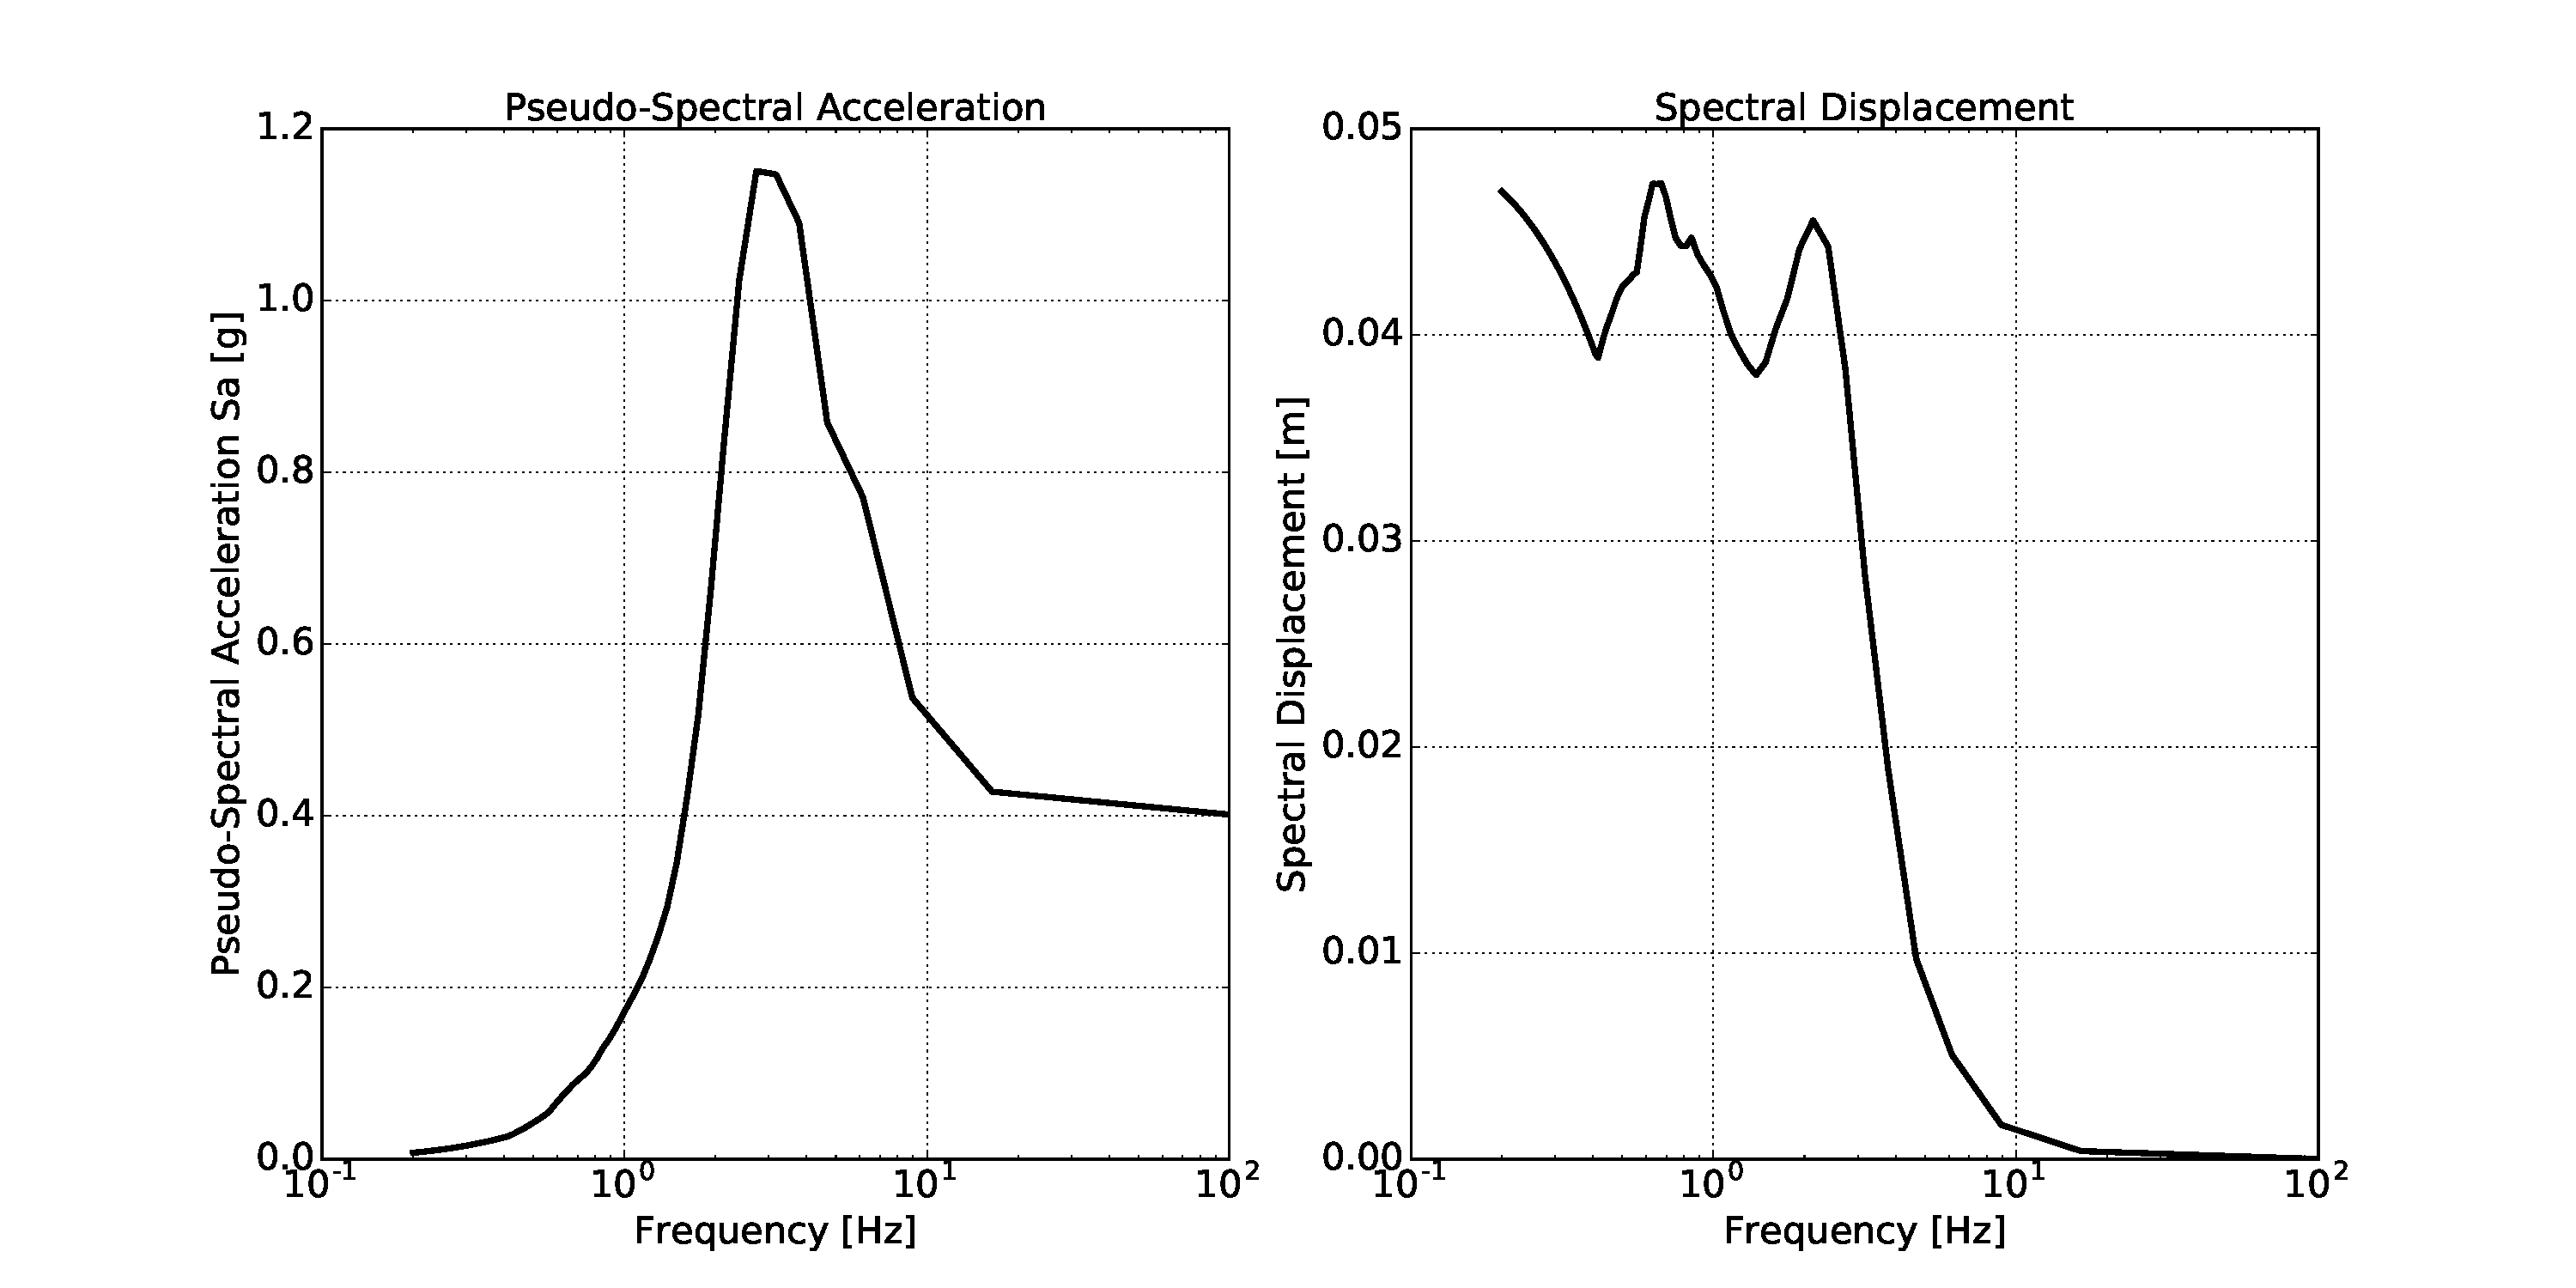
\includegraphics[width = 15cm]{./Figure-files/nonlinear_analysis_steps/soil-structure-3D-ans/shell_structure_motion_node_3195_x_spectrum_freq.pdf}
  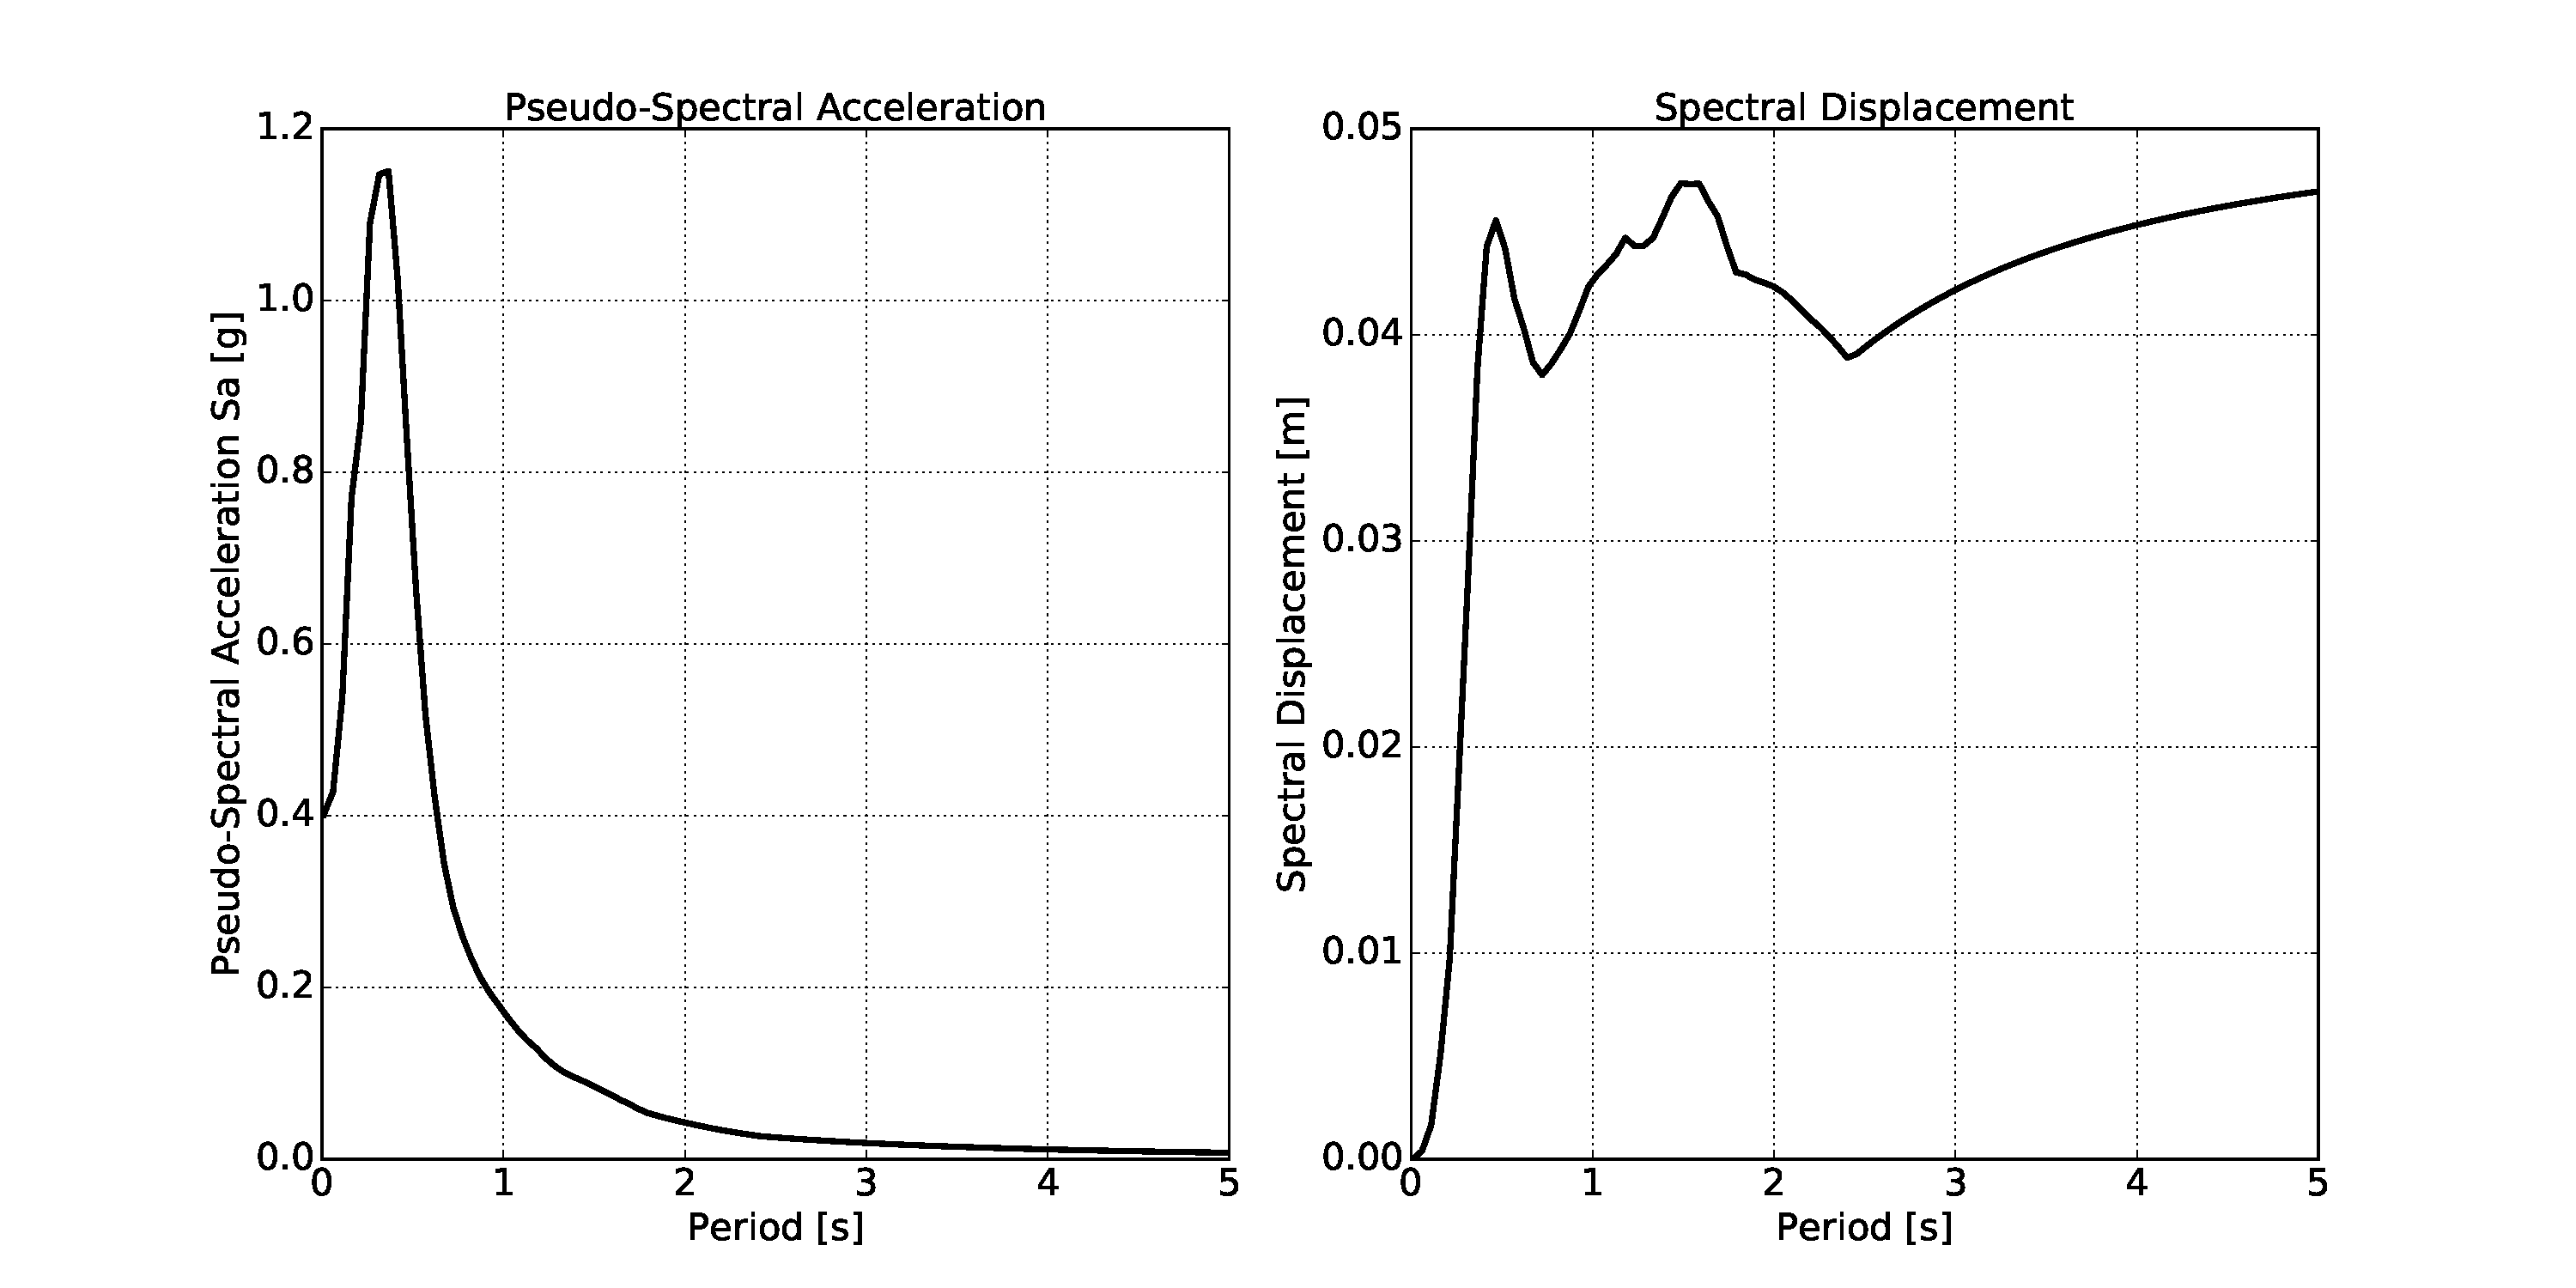
\includegraphics[width = 15cm]{./Figure-files/nonlinear_analysis_steps/soil-structure-3D-ans/shell_structure_motion_node_3195_x_spectrum_period.pdf}
  \caption{Simulation Results: Response Spectrum under 3D motion}
  \label{fig_spectrum_freq_period_time_series_ssi3d_3D_motion}
\end{figure}


% ******************************************************************
% ******************************************************************
% ******************************************************************
\clearpage
\newpage
\section{Structure Analysis without Soil}
\label{structure_only_3D}

\subsection{Eigen Analysis}

The Real-ESSI input files for this example are available 
\href{https://github.com/yuan-energy/Real-ESSI-Short-Course-Examples/tree/master/short-course-examples/nonlinear_analysis_steps/structure/eigen}{HERE}. 
The compressed package of input files is  
\href{https://github.com/yuan-energy/Real-ESSI-Short-Course-Examples/tree/master/short-course-examples/nonlinear_analysis_steps/structure/eigen/eigen.tgz?raw=true}{HERE}. 



The thickness of the shell structure is 2 meters.
The simulation model is shown below.
\begin{figure}[H]
  \centering
  \includegraphics[width = 4cm]{./Figure-files/nonlinear_analysis_steps/structure/eigen/structure-only.png}
  \hspace{2cm}
  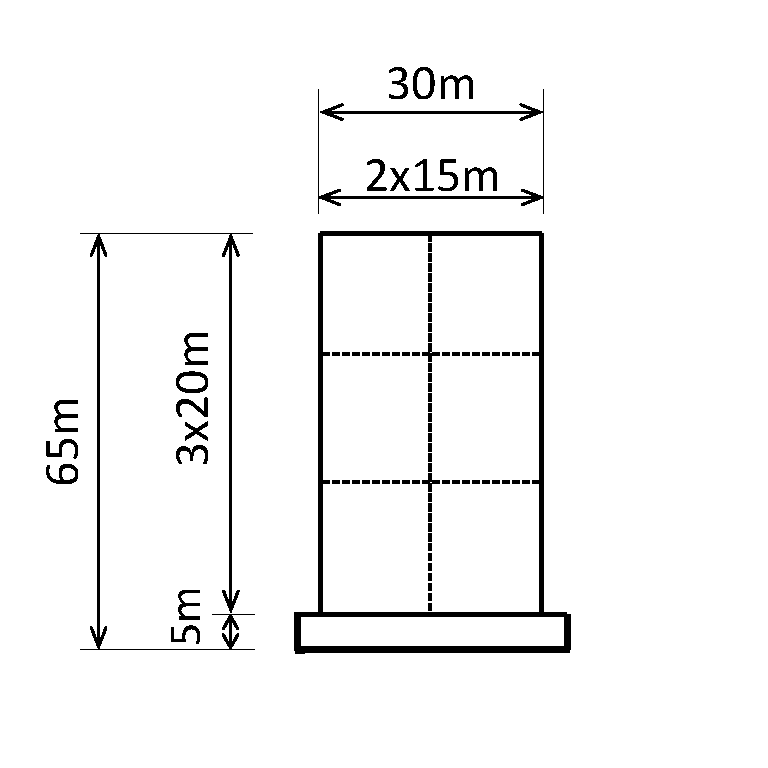
\includegraphics[width = 8cm]{./Figure-files/nonlinear_analysis_steps/structure/eigen/structure_geometry.pdf}
  \caption{Simulation Model}
  \label{fig_simulate_model}
\end{figure}


The eigen results:

\begin{figure}[H]
  \centering
  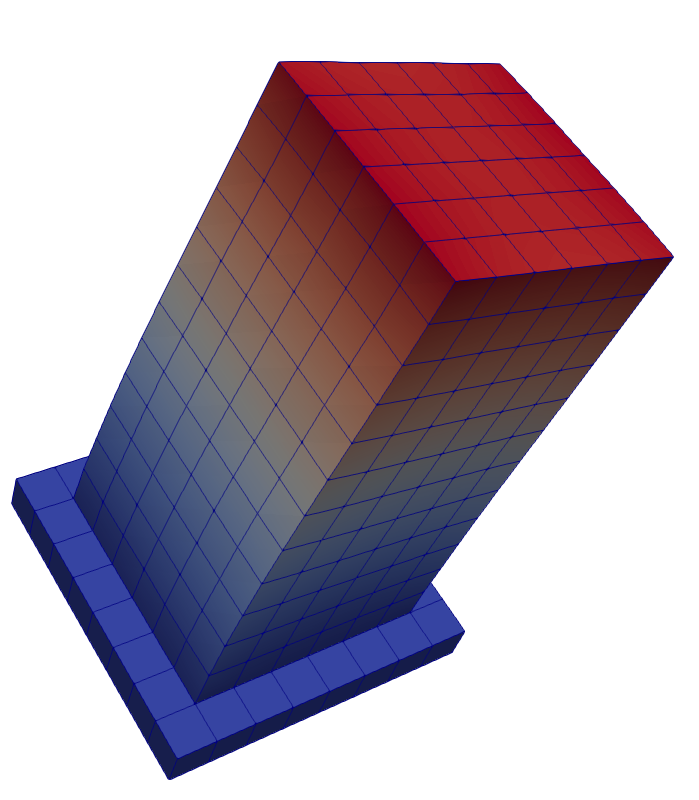
\includegraphics[width = 5cm]{./Figure-files/nonlinear_analysis_steps/structure/eigen/eigen1.png}
  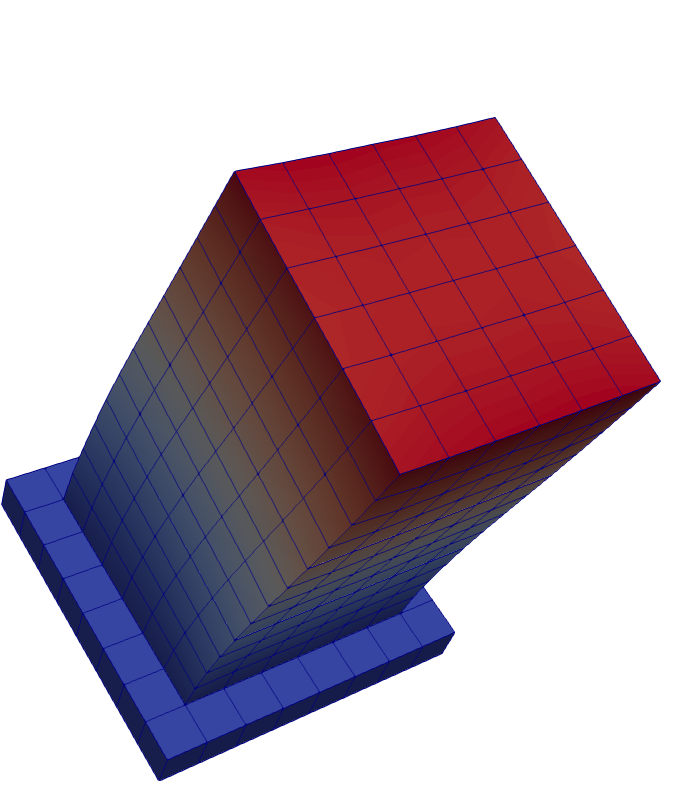
\includegraphics[width = 5cm]{./Figure-files/nonlinear_analysis_steps/structure/eigen/eigen2.png}
  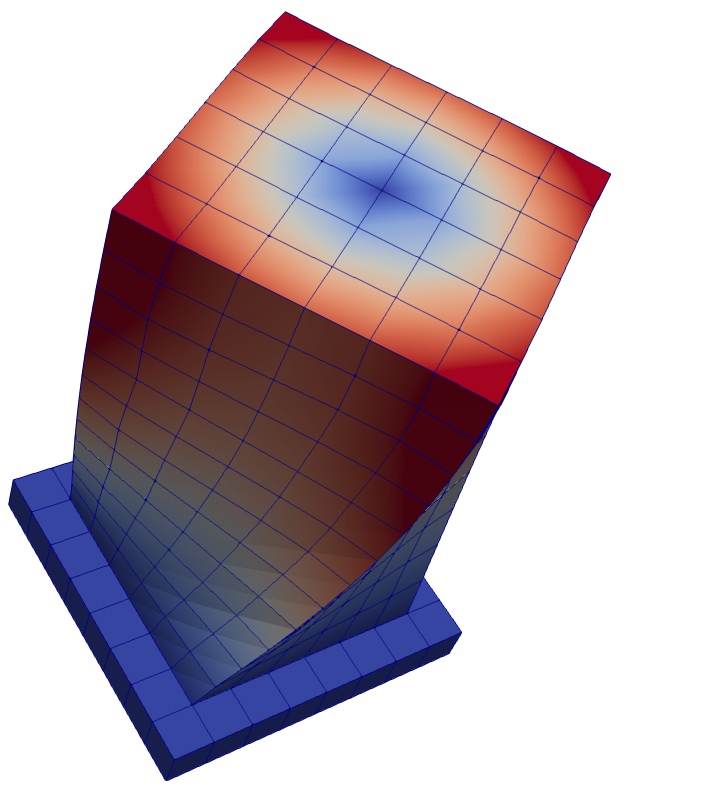
\includegraphics[width = 5cm]{./Figure-files/nonlinear_analysis_steps/structure/eigen/eigen3.png}
  \caption{Eigen Results (Eigen Mode 1 to 3 from left to right)}
  \label{fig_eigen_results_1}
\end{figure}


\begin{figure}[H]
  \centering
  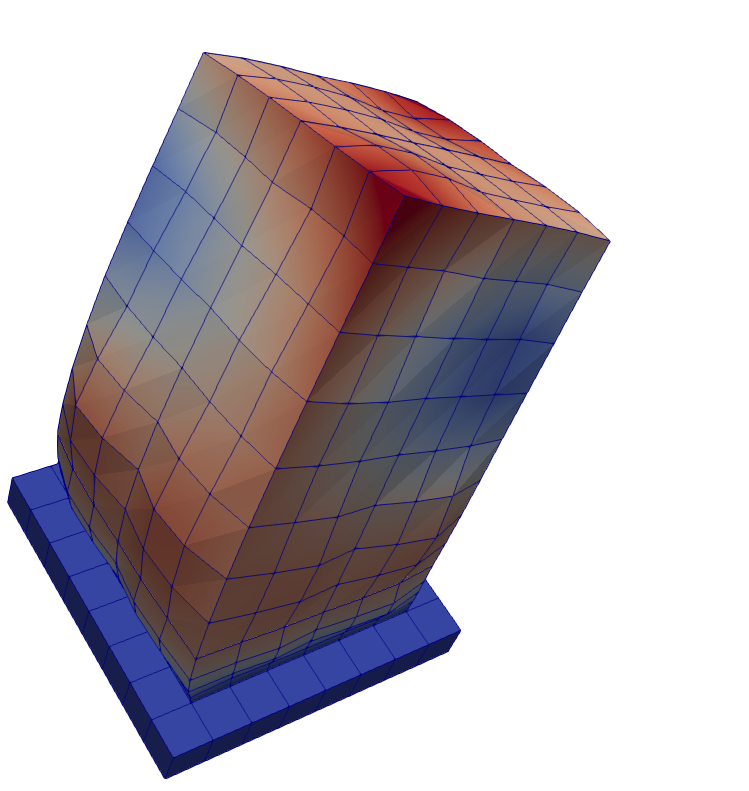
\includegraphics[width = 5cm]{./Figure-files/nonlinear_analysis_steps/structure/eigen/eigen4.png}
  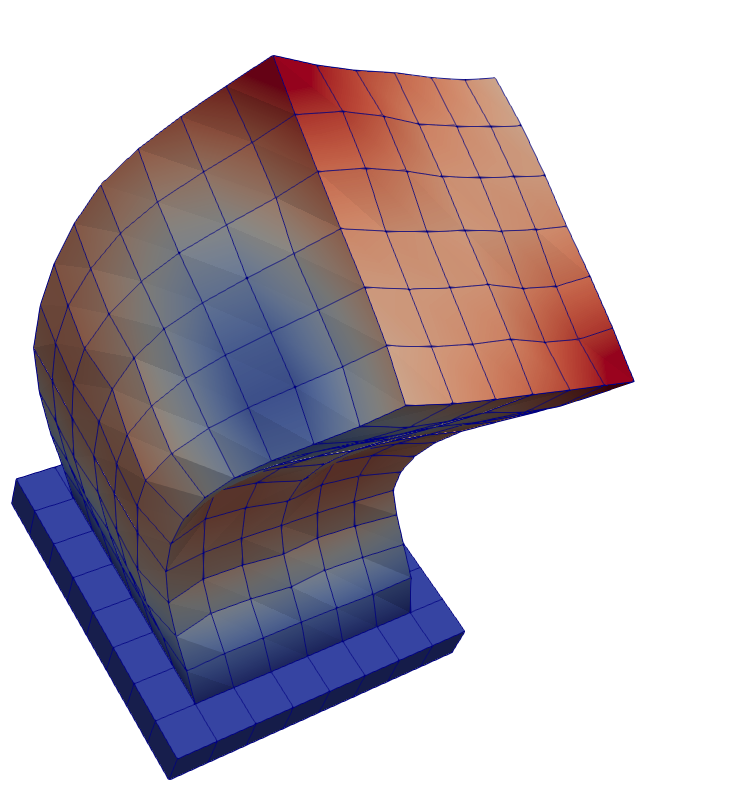
\includegraphics[width = 5cm]{./Figure-files/nonlinear_analysis_steps/structure/eigen/eigen5.png}
  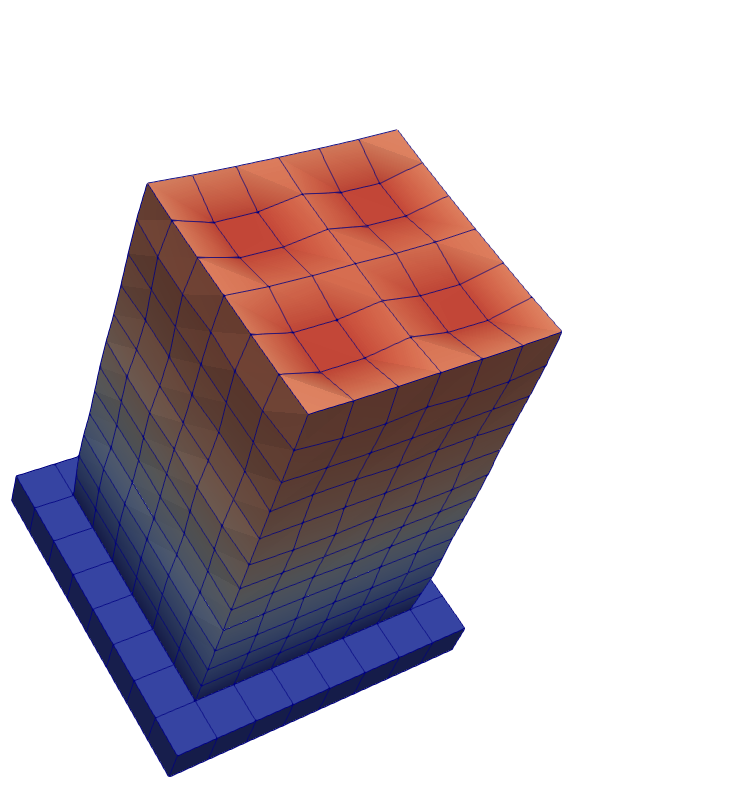
\includegraphics[width = 5cm]{./Figure-files/nonlinear_analysis_steps/structure/eigen/eigen6.png}
  \caption{Eigen Results (Eigen Mode 4 to 6 from left to right)}
  \label{fig_eigen_results_2}
\end{figure}




% ******************************************************************
% ******************************************************************
% ******************************************************************
\clearpage
\newpage
\subsection{Imposed Motion}

The Real-ESSI input files for this example are available 
\href{https://github.com/yuan-energy/Real-ESSI-Short-Course-Examples/tree/master/short-course-examples/nonlinear_analysis_steps/structure/imposed_motion}{HERE}. 
The compressed package of input files is  
\href{https://github.com/yuan-energy/Real-ESSI-Short-Course-Examples/tree/master/short-course-examples/nonlinear_analysis_steps/structure/imposed_motion/imposed_motion.tgz?raw=true}{HERE}. 

The Modeling parameters are listed.
\begin{itemize}
  \item Elastic Material Properties 
  \begin{itemize}
    \item Mass density, $\rho$, \enspace \enspace 2000 $kg/m^3$
    \item Young's modulus, $E$, \enspace \enspace 1.1 GPa
    \item Poisson's ratio, $\nu$, \enspace \enspace 0.1
  \end{itemize}
\end{itemize}


The thickness of the shell structure is 2 meters.
The simulation model is shown below.
\begin{figure}[H]
  \centering
  \includegraphics[width = 4cm]{./Figure-files/nonlinear_analysis_steps/structure/imposed_motion/structure-only.png}
  \hspace{2cm}
  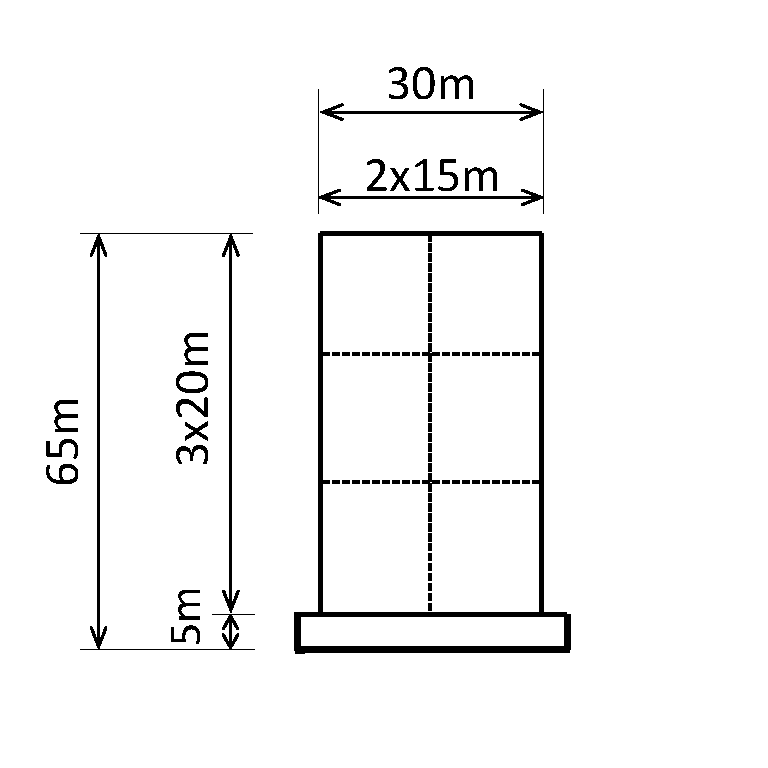
\includegraphics[width = 8cm]{./Figure-files/nonlinear_analysis_steps/structure/eigen/structure_geometry.pdf}
  \caption{Simulation Model}
  \label{fig_simulate_model}
\end{figure}


The simulation results:

\begin{figure}[H]
  \centering
  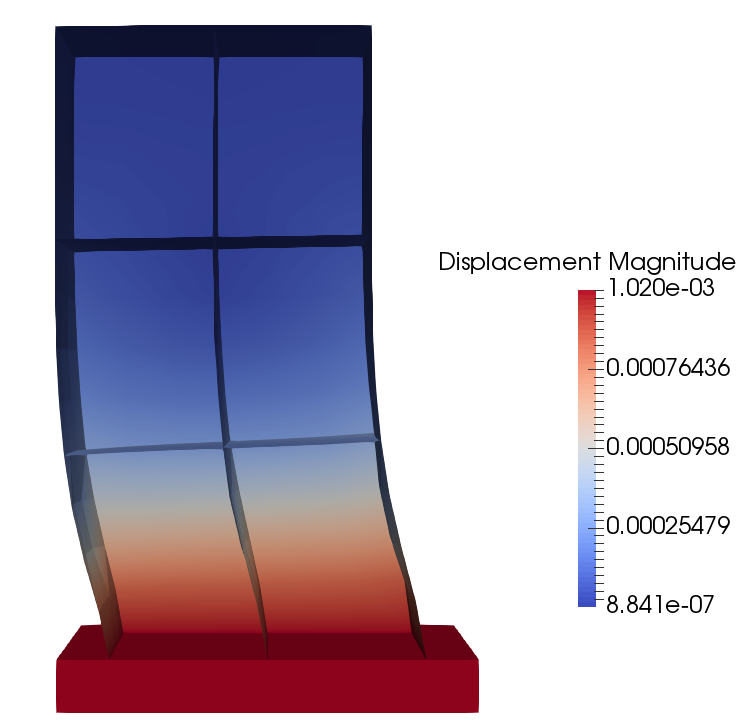
\includegraphics[width = 5cm]{./Figure-files/nonlinear_analysis_steps/structure/imposed_motion/imposed_motion_results.png}
  \caption{Simulation Results}
  \label{fig_simulate}
\end{figure}


